\documentclass{scrartcl} % for better typography/titles; switch to article if need to

% Layout and spacing
\usepackage[margin=1in]{geometry}
\usepackage{setspace}
\onehalfspacing
\usepackage{microtype}

% Typography and language
\usepackage[T1]{fontenc}
\usepackage{lmodern} % this makes a more readable font
\usepackage{csquotes}
\usepackage[english]{babel} % for better hyhenation


% Math
\usepackage{amsmath}
\usepackage{amssymb}
\usepackage{mathtools}

% Tables
\usepackage{booktabs}
\usepackage{tabularx}
\usepackage{threeparttable}
\usepackage{longtable}
\usepackage{pdflscape}
\usepackage{siunitx}
\sisetup{detect-all,group-minimum-digits=4}

% Figures and floats
\usepackage{graphicx}
\usepackage{subcaption}
\usepackage{float}

% Lists and colors
\usepackage{enumitem}
\usepackage{xcolor}

% Hyperlinks and references
\usepackage{hyperref}
\usepackage[nameinlink,capitalise,noabbrev]{cleveref}

% Bibliography
\usepackage[backend=biber,style=authoryear,doi=false,isbn=false,url=true]{biblatex}
\addbibresource{references/adlt-econ580-thesis.bib} % EDIT WITH REFERENCES

\hypersetup{
  colorlinks=true,
  linkcolor=blue,
  citecolor=blue,
  urlcolor=blue
}

% ─── TODO MARKUP ─────────────────────────────────────────────────────────────
% Usage: \TODO{Short label}{Detailed inline note}
% \printtodos prints the Open TODOs section; subsection entries in the TOC
% appear on the second compile after TODOs are added or removed.
\newcounter{todocount}
\newif\iftodospresent
\todospresentfalse
\newwrite\todolistfile
\AtBeginDocument{\immediate\openout\todolistfile=\jobname.tdo}

% Called when the .tdo file is read inside \printtodos.
% Adds a subsection TOC entry linking back to the TODO body location,
% and renders a hyperlinked list item.
\newcommand{\adltodoentry}[2]{%
  \addcontentsline{toc}{subsection}{%
    \protect\hyperlink{todo:#1}{\textcolor{red}{TODO #1: #2}}%
  }%
  \item \hyperlink{todo:#1}{\textbf{TODO #1:} #2}%
}

\newcommand{\TODO}[2]{%
  \stepcounter{todocount}%
  \global\todospresenttrue%
  \hypertarget{todo:\thetodocount}{}%
  \par\noindent%
  \fcolorbox{red}{red!8}{%
    \parbox{\dimexpr\linewidth-2\fboxsep-2\fboxrule\relax}{%
      \textbf{\textcolor{red}{TODO \thetodocount\ ---\ #1}}\\[0.3em]%
      \textcolor{red}{#2}%
    }%
  }\par\medskip%
  \immediate\write\todolistfile{%
    \string\adltodoentry{\thetodocount}{\detokenize{#1}}%
  }%
}

\newcommand{\printtodos}{%
  \immediate\closeout\todolistfile%
  \phantomsection%
  \section*{Open TODOs}%
  \addcontentsline{toc}{section}{\texorpdfstring{\textcolor{red}{Open TODOs}}{Open TODOs}}%
  \iftodospresent%
    \begin{itemize}%
      \input{\jobname.tdo}%
    \end{itemize}%
  \else%
    \textit{No open TODOs.}%
  \fi%
}
% ─────────────────────────────────────────────────────────────────────────────

% TITLE CONFIGURATION
\title{
  \Huge Regulatory Reform and the Composition of FDA Drug Approvals
}

\subtitle{
  \large Evidence on Controlled Substances, Regulatory Incentives, and Pharmaceutical Market Composition
}
\author{
  Alejandro De La Torre \\[0.5em]
  %Advised by Professor [Advisor Name] % EDIT WITH ADVISOR NAME IF APPLICABLE
  \thanks{University of Wisconsin--Madison. Contact: adelatorre2@wisc.edu.\\[0.5em]}
}
\date{\Large April 2026 \\[1em]
\normalsize \href{https://github.com/adelatorre2/adlt-econ580-thesis}{Click here for the latest version.}}



\begin{document}

% COVER PAGE
\maketitle
\begin{abstract}

The Prescription Drug User Fee Act of 1992 (PDUFA) and the Generic Drug User Fee Amendments of 2012 (GDUFA) authorized the FDA to collect industry fees in exchange for binding review-time targets. Standard incentive logic predicts that user-fee acceleration should disproportionately benefit drugs with the largest expected revenue streams, including many controlled substances. I test this hypothesis using the Drugs@FDA database linked to DEA scheduling records (1939--2025, $N = 25{,}908$ original approvals) and estimate interrupted time series, Poisson rate models with exposure, and stacked difference-in-differences specifications. Once group-specific trends are allowed, the estimated effect on the controlled-substance share is indistinguishable from zero for both policies (PDUFA NDA-only IRR $= 1.19$, 95\% CI $[0.59, 2.39]$; GDUFA ANDA-only IRR $= 1.38$, 95\% CI $[0.86, 2.21]$). A separable late-2000s wave of branded abuse-deterrent opioid NDAs explains apparent rate movements in less flexible specifications.

\end{abstract}

\thispagestyle{empty} % to not count the cover page
\newpage
\setcounter{page}{1}

% TABLE OF CONTENTS
\newpage
\tableofcontents
\newpage

% MAIN CONTENT
\section{Introduction}

The Food and Drug Administration is the gatekeeper of the U.S. pharmaceutical market: its approval decisions determine which drugs may be sold, when they reach patients, and what evidence of safety and efficacy is required before market entry \parencite{carpenterINTRODUCTIONGatekeeper2010}. Since 1992, the agency has been partly funded by industry user fees collected in exchange for binding review-time targets. The Prescription Drug User Fee Act (PDUFA) of 1992 and the Generic Drug User Fee Amendments (GDUFA) of 2012 are widely credited with substantially accelerating drug review and changing the incentive environment facing both the FDA and the firms it regulates \parencite{berndtIndustryFundingFDA2005, olsonPDUFAInitialUS2009, berndtGenericDrugUser2018}. They also coincide, in the United States, with one of the largest public-health crises of the past three decades: drug overdose deaths reached approximately 107{,}000 in 2021, with prescription controlled substances playing a prominent role throughout the trajectory of the epidemic \parencite{markDrugOverdoseDeaths2024}.

A large literature studies the consequences of regulatory acceleration. \textcite{berndtIndustryFundingFDA2005} document that PDUFA substantially reduced NDA review times and increased approval rates. \textcite{carpenterDrugreviewDeadlinesSafety2008} show that drugs approved just before PDUFA deadlines exhibit higher rates of subsequent safety-related labeling actions than those approved just after. \textcite{philipsonCostbenefitAnalysisFDA2008} build a welfare framework around the speed--safety tradeoff. \textcite{olsonPDUFAInitialUS2009} and \textcite{olsonFirmCharacteristicsSpeed1997} examine launch behavior and firm-side heterogeneity in pre-PDUFA review times. The accelerated-approval and coverage literature, including \textcite{darrowFDAApprovalRegulation2020} and \textcite{gelladAcceleratedApprovalExpensive2017}, documents how shorter review reduces clinical evidence requirements at approval. A separate body of work in the economics of controlled substances studies the supply side of misuse and diversion: \textcite{alpertSupplySideDrugPolicy2018a}, for example, show that the 2010 abuse-deterrent reformulation of OxyContin reduced prescription opioid misuse but shifted users into illicit markets.

These two literatures have not been joined. Existing studies of user-fee reform identify effects on review times, launch timing, post-market safety, and welfare, but do not ask whether either reform changed the \textit{composition} of approved drugs along the controlled-substance margin. The omission matters because the standard economic argument for why user-fee acceleration should reshape approval composition is straightforward. Faster review compresses the window between approval and patent expiration and therefore raises the present value of approval; the value of that compression is greatest for drugs with the largest expected revenue streams. Branded extended-release and abuse-deterrent controlled substances --- particularly Schedule~II opioid formulations --- occupy precisely this segment of the market: high list prices, long marketing horizons, and limited generic competition during patent protection \parencite{powellHowIncreasingMedical2020}. If user-fee acceleration tilts the field toward high-margin pipelines, controlled substances should be among the most affected categories. The same incentive logic applies, with sign reversed, to the generic-drug margin under GDUFA, where Schedule~II opioid generics historically face higher manufacturing and compliance costs than non-controlled generics. The null hypothesis is straightforward, theory-relevant, and economically interesting: the user-fee channel could plausibly have shifted the composition of approvals.

This paper provides the first systematic test of that hypothesis. Using the complete Drugs@FDA database linked to DEA scheduling records (1939--2025, $N = 25{,}908$ original approvals), I estimate interrupted time series specifications, Poisson rate models with total approvals as exposure, and stacked difference-in-differences specifications around both PDUFA (1992) and GDUFA (2012). Each specification is run on the application-type subsample where the corresponding policy applies most directly --- new drug applications (NDAs) for PDUFA, abbreviated new drug applications (ANDAs) for GDUFA --- and is supplemented with rate-versus-count diagnostics, group-specific linear time trends, and event-study DD designs.

The headline finding is null. In the most flexible specifications --- those that allow controlled-substance and non-controlled-substance approval streams to follow their own linear trends --- the estimated effect of either reform on the CS share of approvals is indistinguishable from zero, with confidence intervals that span both small and economically meaningful effects on either side of the null. For PDUFA on the NDA pathway, the post-policy incidence-rate ratio is $1.19$ with a 95\% confidence interval of $[0.59, 2.39]$. For GDUFA on the ANDA pathway, the corresponding IRR is $1.38$ with a 95\% confidence interval of $[0.86, 2.21]$. The point estimates flip sign across less flexible and more flexible specifications, which is itself diagnostic: when the only thing absorbing pre/post differences is a year fixed effect, post-PDUFA NDA rates appear elevated and post-GDUFA ANDA rates appear depressed, but both shifts are absorbed once group-specific trends accommodate the slower-moving secular changes in pharmaceutical innovation.

A drug-level investigation of the CS-NDA series locates the most economically interpretable confound. Forty-three CS NDAs were approved between 2009 and 2013 --- roughly twice the typical pace of the preceding decade --- and the cluster maps almost one-for-one onto the well-documented wave of branded extended-release and abuse-deterrent opioid formulations of the late 2000s: the reformulated OxyContin (2010), Exalgo (2010), Embeda (2009), Suboxone (2010), Zohydro ER (2012), and related products. The timing is roughly seventeen to twenty-one years after PDUFA enactment, which is inconsistent with a delayed regulatory-incentive response and consistent with a pharmaceutical product cycle that the FDA accommodated rather than caused. Once this episode is allowed to load on its own group-specific trend rather than on the post-PDUFA dummy, the user-fee effect collapses.

Two broader contributions follow. The first is empirical: across a comprehensive panel of FDA approvals over more than eight decades, the controlled-substance composition of the legal pharmaceutical supply does not appear to respond to user-fee-funded review acceleration. The second is interpretive. Negative results in policy economics are sometimes read as evidence that the question was poorly posed; here, the structure of the test --- a theory-relevant prediction, a comprehensive panel, multiple specifications consistent in direction --- suggests instead that the relevant margin operates elsewhere. The pharmaceutical-innovation channel that produced the late-2000s opioid wave appears to have run on firm-level investment decisions and product-cycle dynamics, with FDA review serving as a downstream accommodation rather than an upstream driver. For the design of future regulatory reforms, this implies that user-fee acceleration is unlikely, on its own, to be a useful margin for influencing the controlled-substance content of the legal pharmaceutical supply.

\paragraph{Roadmap.} Section~\ref{sec:background} reviews the institutional background, the relevant literature, and the theory of user-fee incentives. Section~\ref{sec:data} describes the data and variable construction. Section~\ref{sec:strategy} sets out the empirical strategy. Section~\ref{sec:results} reports the main and supplementary results. Section~\ref{sec:discussion} interprets the findings and discusses their limitations. Section~\ref{sec:conclusion} concludes.

\section{Background and Related Literature}
\label{sec:background}

\subsection{Institutional Background}

\paragraph{PDUFA (1992).}
The Prescription Drug User Fee Act, enacted in October 1992, authorized the FDA to collect fees from pharmaceutical manufacturers to supplement congressional appropriations for drug review \parencite{rep.dingellHR5952102ndCongress1992}. In exchange, the agency agreed to binding performance goals specifying median review times for new drug applications. The original PDUFA I (1993--1997) committed the FDA to reviewing standard applications within twelve months and priority applications within six months of receipt, with completion targets phased in over five years. Subsequent reauthorizations --- PDUFA II through VII --- have progressively tightened review-time targets, expanded the user-fee program to biologics, and added post-market safety obligations. The fee structure is renegotiated between the pharmaceutical industry and the FDA before each five-year reauthorization cycle, a feature that has long raised concerns about regulatory capture \parencite{darrowSpeedSafetyIndustry2017}.

PDUFA applies to applications for new molecular entities and new formulations submitted under the NDA pathway. It does not directly govern the Abbreviated New Drug Application (ANDA) pathway for generic drugs, which was created by the Hatch--Waxman Act of 1984 \parencite{rep.waxmanHR360598thCongress1984}. Until 2012, ANDA reviews were funded entirely by congressional appropriations, which contributed to a backlog of thousands of pending generic applications by the late 2000s.

\paragraph{GDUFA (2012).}
The Generic Drug User Fee Amendments, signed in July 2012, extended the user-fee model to generic drug reviews under the ANDA pathway \parencite{researchGDUFA2024}. GDUFA~I (2013--2017) collected fees from generic manufacturers and established performance goals for ANDA review times. A distinguishing feature of the initial GDUFA implementation was a substantial transition period (2013--2014) during which the FDA worked to clear a pre-existing backlog of approximately 2{,}500 unreviewed applications; the performance-goal era for new ANDA submissions effectively began in 2015. GDUFA~II (2018--2022) and GDUFA~III (2023--2027) have further refined the fee structure and review targets. Because 86.6\% of controlled-substance original approvals in this dataset came through the ANDA pathway, GDUFA is arguably the more directly relevant policy for this paper's central question.

\subsection{Theory of User-Fee Incentives}
\label{sec:theory}

The standard economic argument for why user-fee acceleration should change the composition of FDA approvals operates through the present value of approval. Let $V_j$ denote the present value of approval for drug $j$, $\pi_{jt}$ the per-period flow profit between approval and patent expiration, $\delta$ the discount factor, $T_j$ the patent expiration date, and $\tau_j$ the approval date. Then
\[
V_j \;=\; \sum_{t = \tau_j}^{T_j} \delta^{t - \tau_j}\,\pi_{jt}.
\]
A reduction in $\tau_j$ --- the approval date --- raises $V_j$ by extending the marketing window and front-loading the cash-flow stream. The marginal value of one additional period of marketing exclusivity, $\partial V_j / \partial \tau_j$, is increasing in $\pi_{jt}$. Holding patent term fixed, the firms with the most to gain from review acceleration are therefore those with the highest expected per-period profits during the on-patent window.

Three features of the controlled-substance segment plausibly place it above the cross-sectional mean of $\pi_{jt}$ during the relevant period. First, branded extended-release and abuse-deterrent opioid formulations command high list prices and have historically faced limited generic competition under patent protection \parencite{powellHowIncreasingMedical2020}. Second, demand for prescription opioid analgesics in the late twentieth and early twenty-first centuries grew rapidly relative to most non-controlled therapeutic categories, expanding the market in which these drugs competed. Third, the regulatory and reimbursement environment for chronic pain --- the largest indication for branded opioids --- supported broad insurance coverage and clinician adoption, raising effective per-patient revenue. Each of these features makes the theoretical prediction sharper rather than weaker: if the value of accelerated approval scales with expected on-patent profits, branded controlled substances should be near the top of the cross-sectional distribution of value gained from PDUFA.

The same logic, with the sign reversed, applies on the generic margin under GDUFA. Schedule~II generics carry meaningful additional manufacturing, distribution, and security costs --- DEA quota allocations, controlled storage, and Suspicious Order Monitoring requirements raise the fixed and variable costs of producing a controlled-substance generic relative to a non-controlled generic. If user-fee acceleration on the ANDA side reduces approval lags by an equal amount across applications, the resulting present-value boost is a smaller share of total project cost for non-controlled generics with low fixed costs than for controlled-substance generics, biasing the post-GDUFA composition shift toward non-CS ANDAs. Either way, the user-fee margin has a clear theoretical reason to move the controlled-substance share of approvals away from its pre-policy baseline.

A competing hypothesis holds that the operative mechanism behind PDUFA-era review-time improvements is not the demand-side shift created by user fees but the supply-side expansion in FDA review capacity that those fees financed. \textcite{ApprovalTimesNew} argue that the level of FDA staffing and review resources matters more than the source of funding. Under that view, PDUFA improved review-time performance primarily by enabling the FDA to hire and retain expertise, and any composition effect would operate through the supply of review capacity rather than through demand-side incentives for manufacturers. Because both channels were activated simultaneously by PDUFA, the reduced-form approval-side test in this paper does not separate them; what it does is bound the joint effect that any plausible mechanism could have produced through the approval-composition margin.

\subsection{Related Empirical Literature}

\paragraph{PDUFA, review speed, and approval.}
The most direct predecessor is \textcite{berndtIndustryFundingFDA2005}, who use drug-level panel data to show that PDUFA substantially reduced NDA review times and increased approval rates while finding little evidence of increased post-approval withdrawals. \textcite{olsonPDUFAInitialUS2009} examines launch decisions and finds that PDUFA increased the probability of U.S.\ initial launch conditional on development, consistent with the thesis that faster review improves the expected return to development. \textcite{olsonFirmCharacteristicsSpeed1997} documents substantial heterogeneity in pre-PDUFA review times across firm types, suggesting that any compositional effects of user-fee acceleration may depend on which firms were most constrained by review delays before 1992. \textcite{dranoveImportantDrugsReach1994} provide an early analysis of whether important drugs reach the market faster, finding limited evidence of differential queue position by therapeutic value.

\paragraph{Post-market safety.}
\textcite{carpenterDrugreviewDeadlinesSafety2008} exploit the fact that drugs approved just before PDUFA deadlines received less review time than those approved just after, finding that proximity-to-deadline approvals are associated with higher rates of subsequent safety-related labeling changes. \textcite{darrowFDAApprovalRegulation2020} review the broader evidence and argue that expedited pathways have reduced clinical evidence requirements at the time of approval, raising concerns about downstream safety for certain product classes. Both papers are informative about the speed--safety margin but do not address the market-composition question examined here.

\paragraph{Welfare analysis.}
\textcite{philipsonCostbenefitAnalysisFDA2008} develop a formal welfare model of the FDA approval decision and use it to estimate that approval delays under the pre-PDUFA regime imposed large welfare costs. The framework emphasizes the consumer-surplus value of earlier access to beneficial drugs but does not model externalities associated with abuse potential or diversion. That omission is consequential for controlled substances, where the social cost of approval may include downstream misuse spillovers that are not internalized by approving firms or patients.

\paragraph{Generic drugs and GDUFA.}
\textcite{berndtGenericDrugUser2018} provide the first systematic economic analysis of GDUFA, documenting that the reform reduced ANDA review times and approval lags. They also analyze barriers to generic entry and argue that regulatory delays were a significant constraint on competition in the pre-GDUFA era. Their analysis is primarily about generic market structure and does not focus on controlled-substance composition.

\paragraph{Controlled substances and opioid supply.}
\textcite{alpertSupplySideDrugPolicy2018a} show that the introduction of abuse-deterrent OxyContin in 2010 reduced prescription opioid misuse but was followed by substitution to heroin, illustrating supply-side spillovers in controlled-substance markets. \textcite{powellEVOLVINGCONSEQUENCESOXYCONTIN2021} extend this analysis through the fentanyl era. Neither paper studies the FDA approval side of the supply chain. This paper contributes by examining whether the upstream regulatory decision environment shaped the composition of what entered the market.

\paragraph{Gap.}
No existing study examines whether PDUFA or GDUFA changed the controlled-substance share of FDA approvals. The literature has studied review times, launch timing, post-market safety, and welfare under PDUFA, and market structure under GDUFA; the composition question has not been addressed. This paper fills that gap and reports a precisely estimated null whose magnitude bounds, rather than merely fails to reject, the user-fee composition hypothesis.

\section{Data}
\label{sec:data}

\subsection{Sources}

\paragraph{FDA Drugs@FDA.}
The primary data source is the Drugs@FDA flat-file database, downloaded from the FDA website in March 2026 \parencite{researchDrugsFDADataFiles2026}. The database consists of twelve tab-delimited tables covering all FDA drug application and submission records from 1939 to the present. The core tables are \texttt{Applications} (one row per application, keyed by \texttt{ApplNo}), \texttt{Submissions} (one row per submission event, keyed by \texttt{ApplNo + SubmissionType + SubmissionNo}), and \texttt{Products} (product-level details linked to applications). Supporting tables cover submission classification codes, action types, document types, marketing status, and therapeutic equivalence codes.

I restrict attention to original approvals---applications with at least one submission classified as a new original application (\texttt{SubmissionClass} = ORIG or equivalent)---and collapse to one row per application. This yields the drug-level panel of $N = 25{,}908$ observations used throughout the paper.

\paragraph{DEA controlled-substance reference.}
Controlled-substance status is determined by linking each FDA application to the DEA's official list of scheduled controlled substances \parencite{DrugScheduling}. The linkage is ingredient-based: I match the active ingredient(s) associated with each FDA application to the DEA scheduling reference using a combination of exact-name matching, partial-string matching, and manual review. The match is conservative---only ``confident scheduled'' matches (ingredients with a clear one-to-one mapping to a DEA schedule) are classified as controlled substances in the primary analysis. Uncertain candidates and \texttt{List~I} chemicals are excluded from the main CS indicator but appear in a broad-definition sensitivity check.

An important limitation of this approach is that the DEA linkage reflects \textit{current} scheduling status, not historical status at the time of approval. Because scheduling can change over time, the current-status linkage may misclassify some drugs approved before they were scheduled and include others that were rescheduled after approval. The direction of the resulting bias is ambiguous but is likely small for the primary CS indicator, which focuses on commonly scheduled substances that have been on DEA schedules for decades.

\subsection{Variable Construction}

\paragraph{Outcome.}
The primary outcome is the annual share of original approvals that are controlled substances, constructed separately for the full sample, NDA-only, and ANDA-only subsamples. Let $y_t$ denote the CS share in year $t$:
\[
y_t = \frac{\text{CS approvals}_t}{\text{Total approvals}_t}
\]
where ``CS approvals'' counts applications matched to a confident DEA schedule.

\paragraph{Application type.}
The variable \texttt{appltype\_str} from the Drugs@FDA Applications table distinguishes NDA (new drug applications for brand-name and certain generic drugs), ANDA (abbreviated new drug applications for generic drugs), and BLA (biologics license applications). In the annual panel, 86.6\% of CS approvals are ANDAs, reflecting the large volume of generic controlled-substance approvals---primarily opioid, benzodiazepine, and stimulant generics---processed through the ANDA pathway.

\paragraph{Policy timing.}
Three binary indicators capture the major policy transitions:
\begin{itemize}[noitemsep]
  \item \texttt{post\_pdufa}: equals 1 for approval years 1993 and later.
  \item \texttt{post\_gdufa}: equals 1 for approval years 2015 and later (the post-performance-goal era, excluding the 2013--2014 backlog-washout transition).
  \item \texttt{post\_hatchwaxman}: equals 1 for approval years 1985 and later.
\end{itemize}

\paragraph{Event time.}
For event-study specifications, event time is measured relative to the policy year. For PDUFA, $\tau = t - 1992$, with the reference year set to $\tau = -1$ (1991). For GDUFA, $\tau = t - 2012$, with reference year $\tau = -1$ (2011). End-caps are applied at $[-20, +30]$ for PDUFA and $[-10, +10]$ for GDUFA to limit sensitivity to sparse years far from the event.

\subsection{Panel Structure}

The drug-level panel covers 1939--2025. For the main event-study analysis, I aggregate to annual cells. The PDUFA specifications use the full 1939--2025 annual panel; the GDUFA specifications use the ANDA-only subsample covering 1984--2025. Stacked difference-in-differences specifications reshape the annual panel into a two-row-per-year format (CS group vs.\ non-CS group) as described in Section~\ref{sec:strategy}.

\subsection{Summary Statistics}

Table~\ref{tab:era_summary} reports the number of approvals and CS share by PDUFA reauthorization era. Several patterns stand out. First, the aggregate CS share is broadly stable in the 7--10\% range across most eras, with a modest elevation in PDUFA II (2003--2007, 10.8\%) and a sharp decline in PDUFA VII (2022--present, 4.5\%). Second, ANDA volume grew dramatically after Hatch--Waxman (1984), accounting for the large increase in total approvals from the pre-Hatch--Waxman to post-Hatch--Waxman eras. Third, the NDA count has been relatively stable at 300--550 per five-year period across the PDUFA era.

Table~\ref{tab:prepost_summary} provides pre/post comparisons for PDUFA and GDUFA. The aggregate CS share fell from 9.6\% pre-PDUFA to 7.3\% post-PDUFA. Among NDAs, the CS share was nearly identical in the two periods (5.1\% pre vs.\ 5.3\% post). Among ANDAs, the CS share fell from 14.3\% to 8.1\%, driven largely by the post-Hatch-Waxman expansion in non-CS generic approvals. For GDUFA, the ANDA CS share fell from 10.8\% (pre-GDUFA, $\leq 2012$) to 7.1\% (post-GDUFA performance-goal era, $\geq 2015$).

\begin{table}[htbp]
\centering
\begin{threeparttable}
\caption{Original FDA Approvals by PDUFA Era}
\label{tab:era_summary}
\small
\begin{tabular}{lrrrrrr}
\toprule
Era & Years & Total & NDA & ANDA & CS & CS Share \\
\midrule
Pre-Hatch--Waxman & $\leq$1984 & 4,270 & 1,488 & 2,005 & 392 & 9.2\% \\
Post-HW, Pre-PDUFA & 1985--1992 & 3,031 & 676 & 2,133 & 309 & 10.2\% \\
PDUFA I & 1993--1997 & 1,525 & 467 & 964 & 114 & 7.5\% \\
PDUFA II & 1998--2002 & 1,662 & 422 & 1,187 & 179 & 10.8\% \\
PDUFA III & 2003--2007 & 2,281 & 429 & 1,775 & 166 & 7.3\% \\
PDUFA IV & 2008--2012 & 2,761 & 394 & 2,300 & 210 & 7.6\% \\
PDUFA V & 2013--2017 & 3,464 & 551 & 2,830 & 268 & 7.7\% \\
PDUFA VI & 2018--2022 & 4,380 & 542 & 3,715 & 316 & 7.2\% \\
PDUFA VII & 2023+ & 2,534 & 308 & 2,113 & 113 & 4.5\% \\
\midrule
Total & 1939--2025 & 25,908 & 4,277 & 19,022 & 2,067 & 8.0\% \\
\bottomrule
\end{tabular}
\begin{tablenotes}
\footnotesize
\item Source: Drugs@FDA (March 2026 extract) linked to DEA controlled-substance schedules.
\item CS = Controlled Substance (conservative: confident DEA scheduled matches only).
\item NDA counts exclude BLA (biologics) and unknown application types.
\end{tablenotes}
\end{threeparttable}
\end{table}

\begin{table}[htbp]
\centering
\begin{threeparttable}
\caption{Pre/Post Comparisons: PDUFA (1992) and GDUFA (2012)}
\label{tab:prepost_summary}
\small
\begin{tabular}{lrrrrrr}
\toprule
 & Total & NDA & ANDA & CS & CS/NDA & CS/ANDA \\
\midrule
\multicolumn{7}{l}{\textit{Panel A: PDUFA}} \\
Pre-PDUFA ($\leq$1992) & 7,301 & 2,164 & 4,138 & 701 & 5.1\% & 14.3\% \\
Post-PDUFA ($\geq$1993) & 18,607 & 3,113 & 14,884 & 1,366 & 5.3\% & 8.1\% \\
\midrule
\multicolumn{7}{l}{\textit{Panel B: GDUFA (ANDA-only)}} \\
Pre-GDUFA ($\leq$2012) & 8,359 & --- & 8,359 & 858 & --- & 10.8\% \\
Post-GDUFA ($\geq$2015) & 7,830 & --- & 7,830 & 556 & --- & 7.1\% \\
\bottomrule
\end{tabular}
\begin{tablenotes}
\footnotesize
\item GDUFA transition years (2013--2014) are excluded from Panel B.
\item Pre-PDUFA period includes both pre-Hatch--Waxman and post-HW/pre-PDUFA years.
\end{tablenotes}
\end{threeparttable}
\end{table}

\subsection{Limitations}

Several data limitations bear on the interpretation of results. First, the DEA linkage reflects current scheduling status, not historical status at the time of approval. Second, the Drugs@FDA database is approval-centered: failed and withdrawn applications are not observed, which limits the ability to study the intensive margin of manufacturer drug development decisions. Third, the ingredient-level linkage may misclassify combination products with both controlled and non-controlled ingredients; the variable \texttt{is\_multi\_ingredient} flags these cases (8\% of CS approvals). Fourth, review-priority coding (\texttt{review\_priority}) is available but unstable over time and is not used as a main outcome. Fifth, the annual series is a single national time series without cross-sectional variation in the main specifications, limiting the credibility of causal inference.

\section{Empirical Strategy}
\label{sec:strategy}

\subsection{Research Design}

The ideal experiment would randomly assign PDUFA or GDUFA implementation across otherwise identical regulatory environments and observe the resulting change in the controlled-substance share of approvals. In practice, both policies were enacted at single national dates and applied to all drug approvals simultaneously, so there is no cross-sectional control group in the standard sense. The analysis therefore relies on time-series comparisons---interrupted time series (ITS) and difference-in-differences (DD) designs---with pre-policy trends serving as the counterfactual for the post-policy period. I treat the estimates as policy-diagnostic first-pass evidence rather than as point-identified causal effects.

\subsection{Interrupted Time Series (ITS)}

The primary specification is a linear ITS estimated on the annual CS-share series:
\begin{equation}
\label{eq:its}
y_t = \alpha + \beta_1 \cdot \text{post}_t + \beta_2 \cdot t + \beta_3 \cdot (\text{post}_t \times t) + \varepsilon_t
\end{equation}
where $y_t$ is the annual CS share in year $t$, $\text{post}_t$ is the post-policy indicator, and the interaction $\text{post}_t \times t$ allows the post-policy trend to differ from the pre-policy trend. The coefficient $\beta_1$ estimates the level shift at the policy date; $\beta_3$ estimates the change in slope. The ITS is estimated separately for PDUFA (1993) and GDUFA (2015). For PDUFA, the sample is restricted to 1970--2025 to focus on the relevant policy window; for GDUFA, the ANDA-only series is used and 2013--2014 are excluded to isolate the backlog-washout transition.

\subsection{Poisson Rate Model}

Because the annual CS share is a proportion bounded between 0 and 1 and the numerator (count of CS approvals) is non-negative, the linear probability model in equation~\eqref{eq:its} may fit poorly in eras with very low or very high shares. I therefore also estimate a Poisson regression treating the annual CS count as the dependent variable and the total annual approval count as an exposure offset:
\begin{equation}
\label{eq:poisson}
\log E[\text{CS}_t] = \alpha + \gamma \cdot \text{post}_t + \log(\text{Total}_t)
\end{equation}
where $\exp(\hat{\gamma})$ is the incidence-rate ratio (IRR) for the post-policy period relative to pre-policy, holding the total approval volume constant. Equation~\eqref{eq:poisson} and its variants add year fixed effects or linear time trends to absorb secular changes in the composition of approvals. All Poisson models use heteroskedasticity-robust standard errors.

\subsection{Stacked Difference-in-Differences}

To increase transparency about the shape of the post-policy change, I also estimate a stacked difference-in-differences specification. For each policy, I reshape the annual panel into a two-row-per-year dataset in which one observation represents CS approvals and the other represents non-CS approvals in each year:
\begin{equation}
\label{eq:dd}
\log E[n_{gt}] = \alpha_g + \lambda_t + \delta \cdot (\text{CS}_g \times \text{post}_t) + \log(\text{Total}_t)
\end{equation}
where $g \in \{\text{CS}, \text{non-CS}\}$ indexes the group, $\alpha_g$ is a group fixed effect, $\lambda_t$ is a year fixed effect, and $\delta$ is the DD coefficient of interest. The post indicator $\text{post}_t$ drops out of the year-FE specification by collinearity. The Poisson DD is estimated with exposure $\text{Total}_t$; $\exp(\hat{\delta})$ is the IRR comparing the relative change in CS approvals to non-CS approvals after the policy. Linear (levels) and inverse hyperbolic sine (IHS) specifications are also estimated for robustness.

\subsection{Event-Study DD}

To examine the dynamics of any post-policy change and test for pre-policy parallel trends, I estimate an event-study version of the DD:
\begin{equation}
\label{eq:eventstudy}
\log E[n_{g\tau}] = \alpha_g + \sum_{\tau \neq -1} \theta_\tau \cdot (\text{CS}_g \times \mathbf{1}[\tau]) + \log(\text{Total}_{g\tau})
\end{equation}
where $\tau$ is event time (calendar year relative to the policy date), and $\theta_\tau$ is the group-specific coefficient at each event-time bin. End-caps are applied at $\tau \in [-20, +30]$ for PDUFA and $\tau \in [-10, +10]$ for GDUFA. The reference period is $\tau = -1$ (the year before each policy). Under the parallel-trends assumption, $\theta_\tau = 0$ for all $\tau < 0$; a pattern of pre-policy zeros followed by post-policy deviations from zero would constitute evidence of a treatment effect \parencite{millerIntroductoryGuideEvent2023}. % TODO: verify citation

\subsection{Threats to Identification}

Three threats to identification are particularly relevant in this context.

\textbf{Confounders contemporaneous with policy.} Both PDUFA (1992) and GDUFA (2012) were enacted at times when other forces were simultaneously reshaping the pharmaceutical market. PDUFA coincided with a period of rapid expansion in ANDA volume following Hatch--Waxman, which could confound any composition effect by diluting non-CS approvals. GDUFA coincided with a surge in generic applications filed to capture expiring patents from the 2005--2012 ``patent cliff.'' I address this by using application-type-specific subsamples (NDA-only for PDUFA, ANDA-only for GDUFA) and by including year fixed effects where applicable.

\textbf{Opioid product cycle (2009--2013).} A spike in Schedule~II NDA approvals around 2009--2013 is visible in the data and drives the apparent post-PDUFA effect in some specifications. Section~\ref{sec:results_nda} and Section~\ref{sec:discussion} document that this spike reflects a specific industry product cycle---the wave of extended-release and abuse-deterrent branded opioid formulations (OxyContin reformulation, Exalgo, Embeda, Suboxone)---rather than a sustained PDUFA-induced composition shift. The event-study design is helpful for diagnosing this: a genuine PDUFA effect should appear near $\tau = 0$ (1992--1993), not 17--19 years later.

\textbf{Single time series.} The national-level panel has only one observation per year, so the effective sample size for time-series inference is small (roughly 50--85 years depending on the specification). Standard errors based on heteroskedasticity alone may understate uncertainty; inference should be treated with appropriate caution.

\subsection{What the Design Can and Cannot Show}

This design can characterize the \textit{reduced-form association} between PDUFA/GDUFA and the controlled-substance share of approvals. A finding of no effect would be informative: it would indicate that user-fee-funded regulatory acceleration did not systematically tilt the composition of approvals toward controlled substances. A finding of a positive effect would be consistent with the regulatory-incentive hypothesis but would not rule out confounding by contemporaneous trends.

What the design \textit{cannot} show is whether any composition change affected downstream misuse, diversion, or overdose mortality. That would require linking the approval-side estimates to prescribing data and ultimately to health outcomes---a step outside the scope of this paper. The contribution is upstream: characterizing the approval-side composition effect (or lack thereof) is a necessary first step before studying downstream consequences.

\section{Results}
\label{sec:results}

\subsection{Descriptive Trends}

Figure~\ref{fig:cs_share_full} plots the annual share of original FDA approvals classified as controlled substances from 1939 through 2025. Three features stand out. First, the share fluctuates broadly in the 5--15\% range over the full sample, with no visually obvious structural break at PDUFA (1992). Second, the series exhibits substantial year-to-year noise in the early portion of the sample, when annual approval counts were small. Third, a moderate elevation is visible from roughly 2009 to 2012, which Section~\ref{sec:results_spike} documents as a separable phenomenon.

\begin{figure}[htbp]
\centering
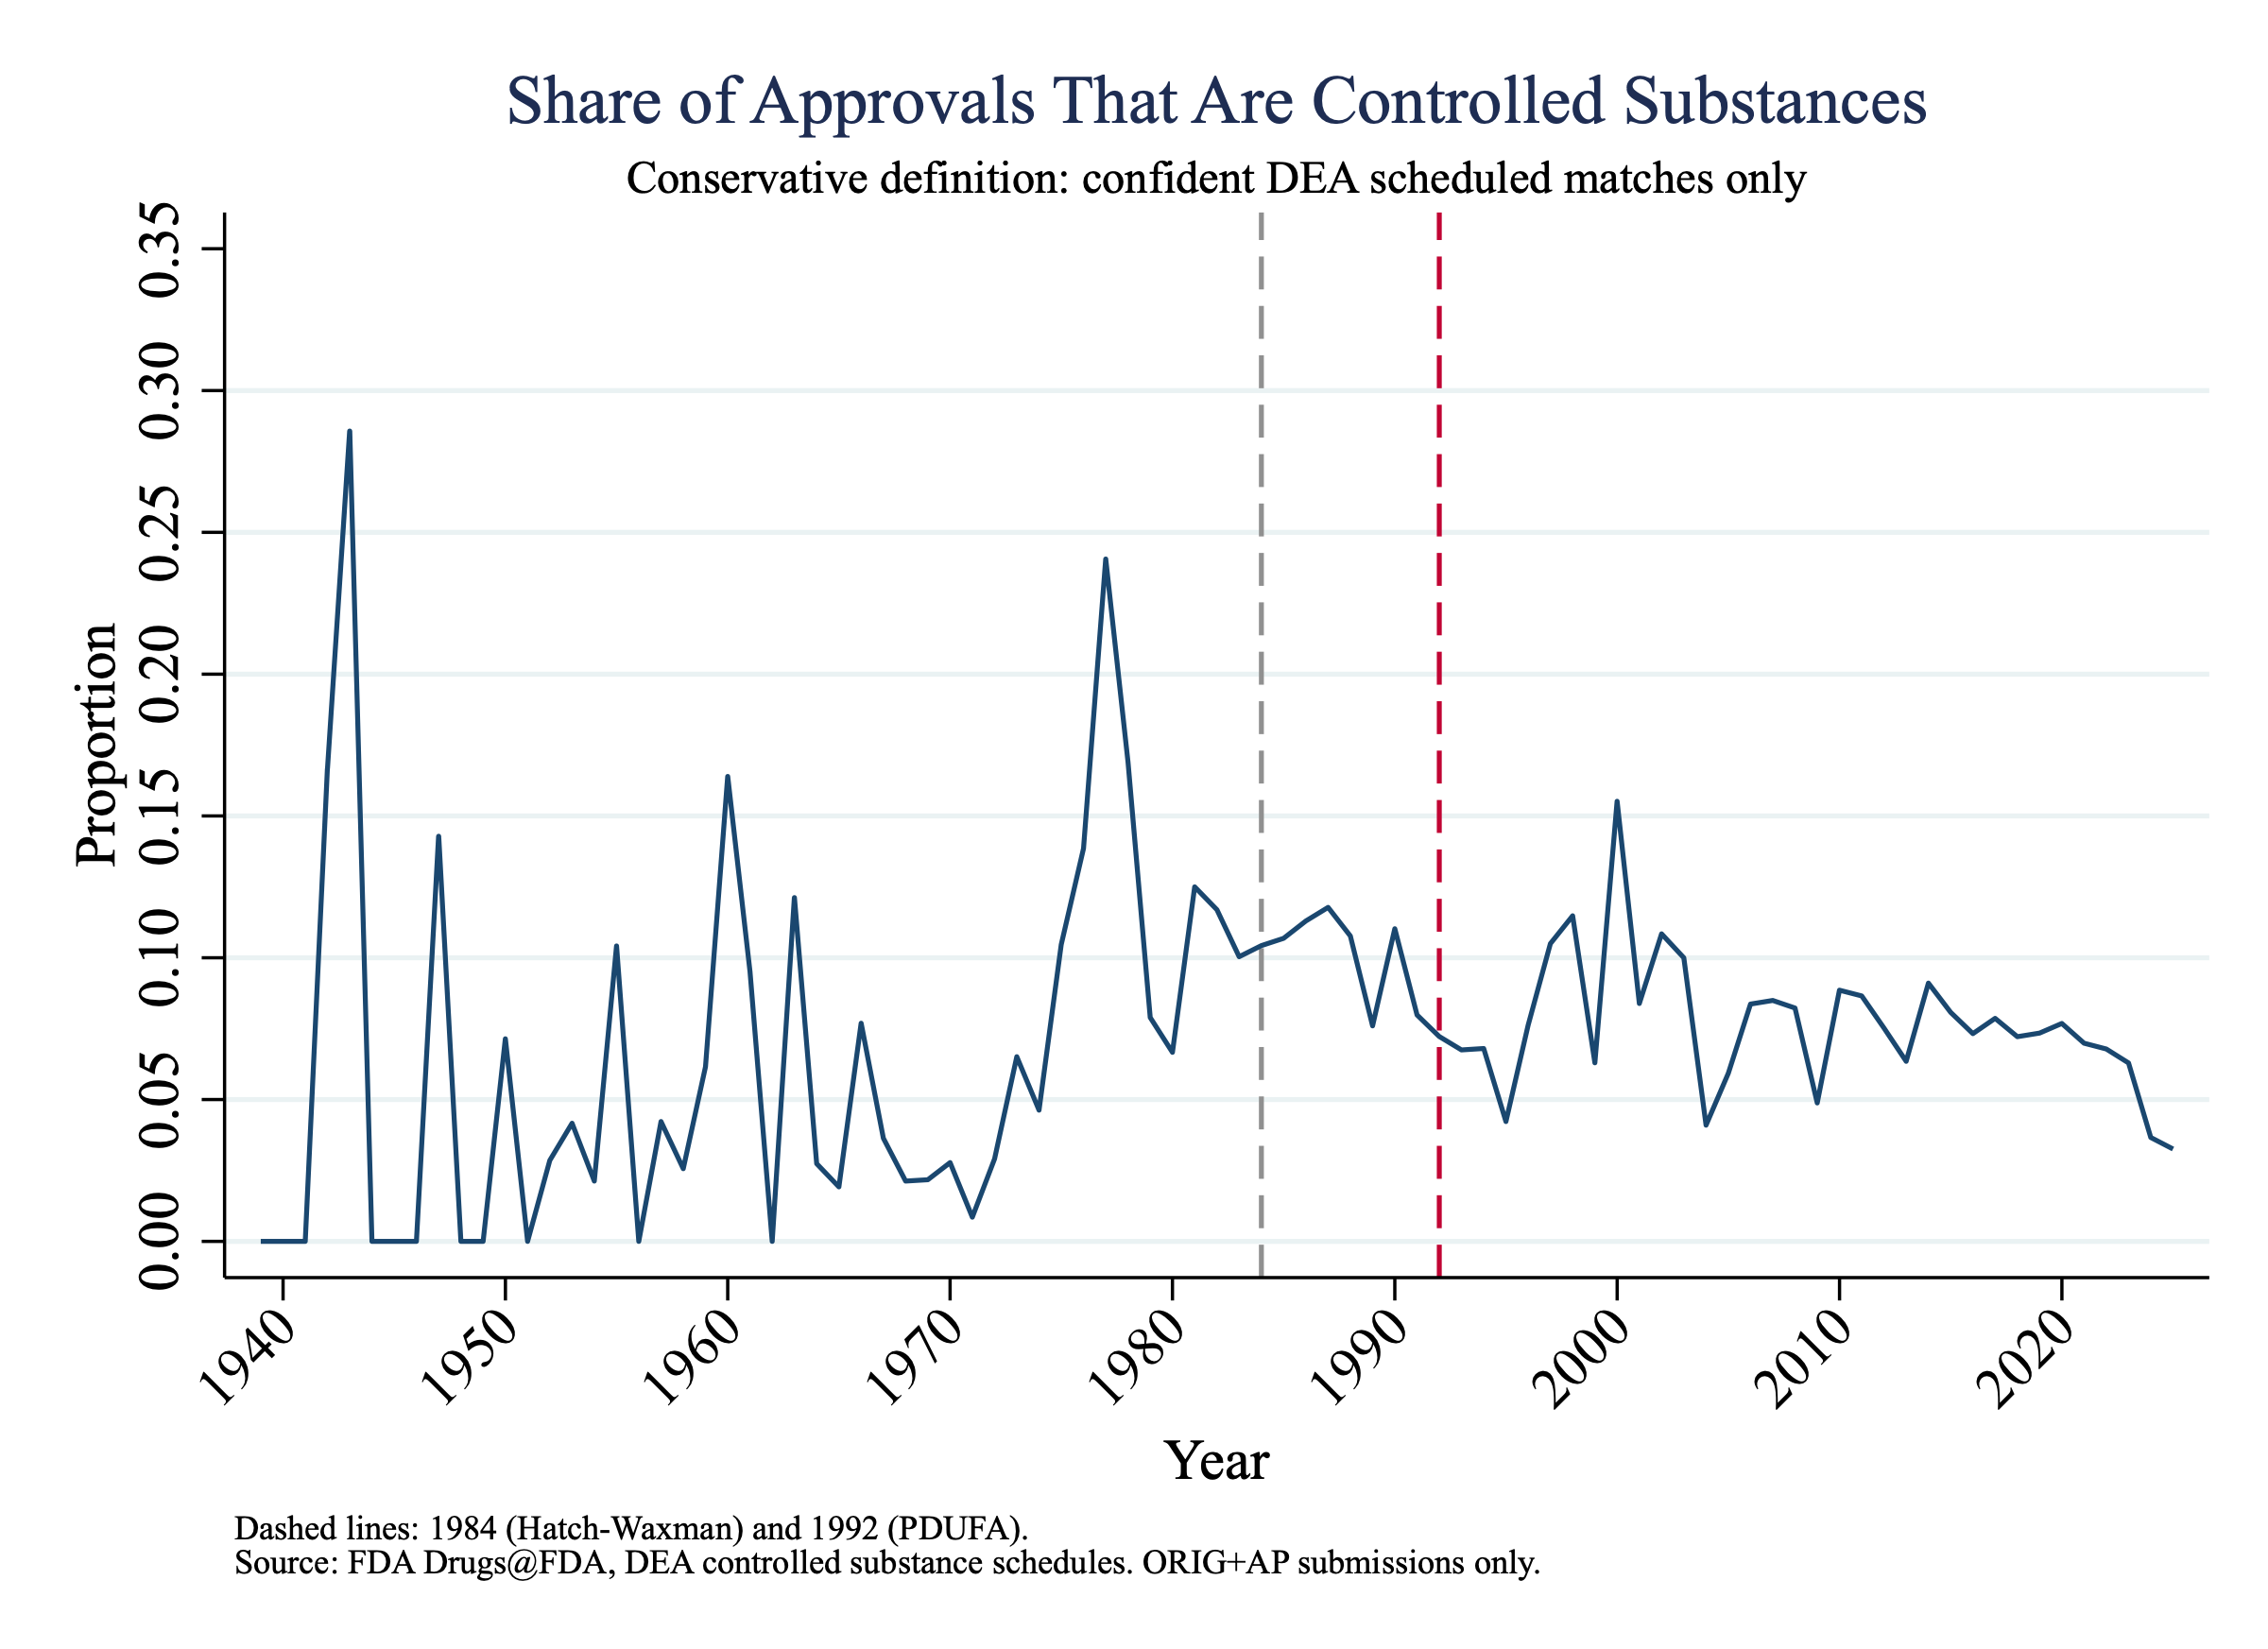
\includegraphics[width=0.92\textwidth]{../output/figures/stata/fig_cs_share.png}
\caption{Annual controlled-substance share of FDA original approvals, 1939--2025. Conservative definition: confident DEA scheduled matches only. Dashed vertical lines mark 1984 (Hatch--Waxman), 1992 (PDUFA), and 2012 (GDUFA).}
\label{fig:cs_share_full}
\end{figure}

Figure~\ref{fig:cs_share_by_type} disaggregates the CS share by application type. The NDA CS share fluctuates narrowly around 5--8\% throughout the sample with no visible trend break at PDUFA. The ANDA CS share is higher --- peaking near 20\% in the early 1980s --- and declines after Hatch--Waxman as the expansion in non-CS generic approvals dilutes the CS share. Years with fewer than five NDA or ANDA approvals are excluded to suppress noise.

\begin{figure}[htbp]
\centering
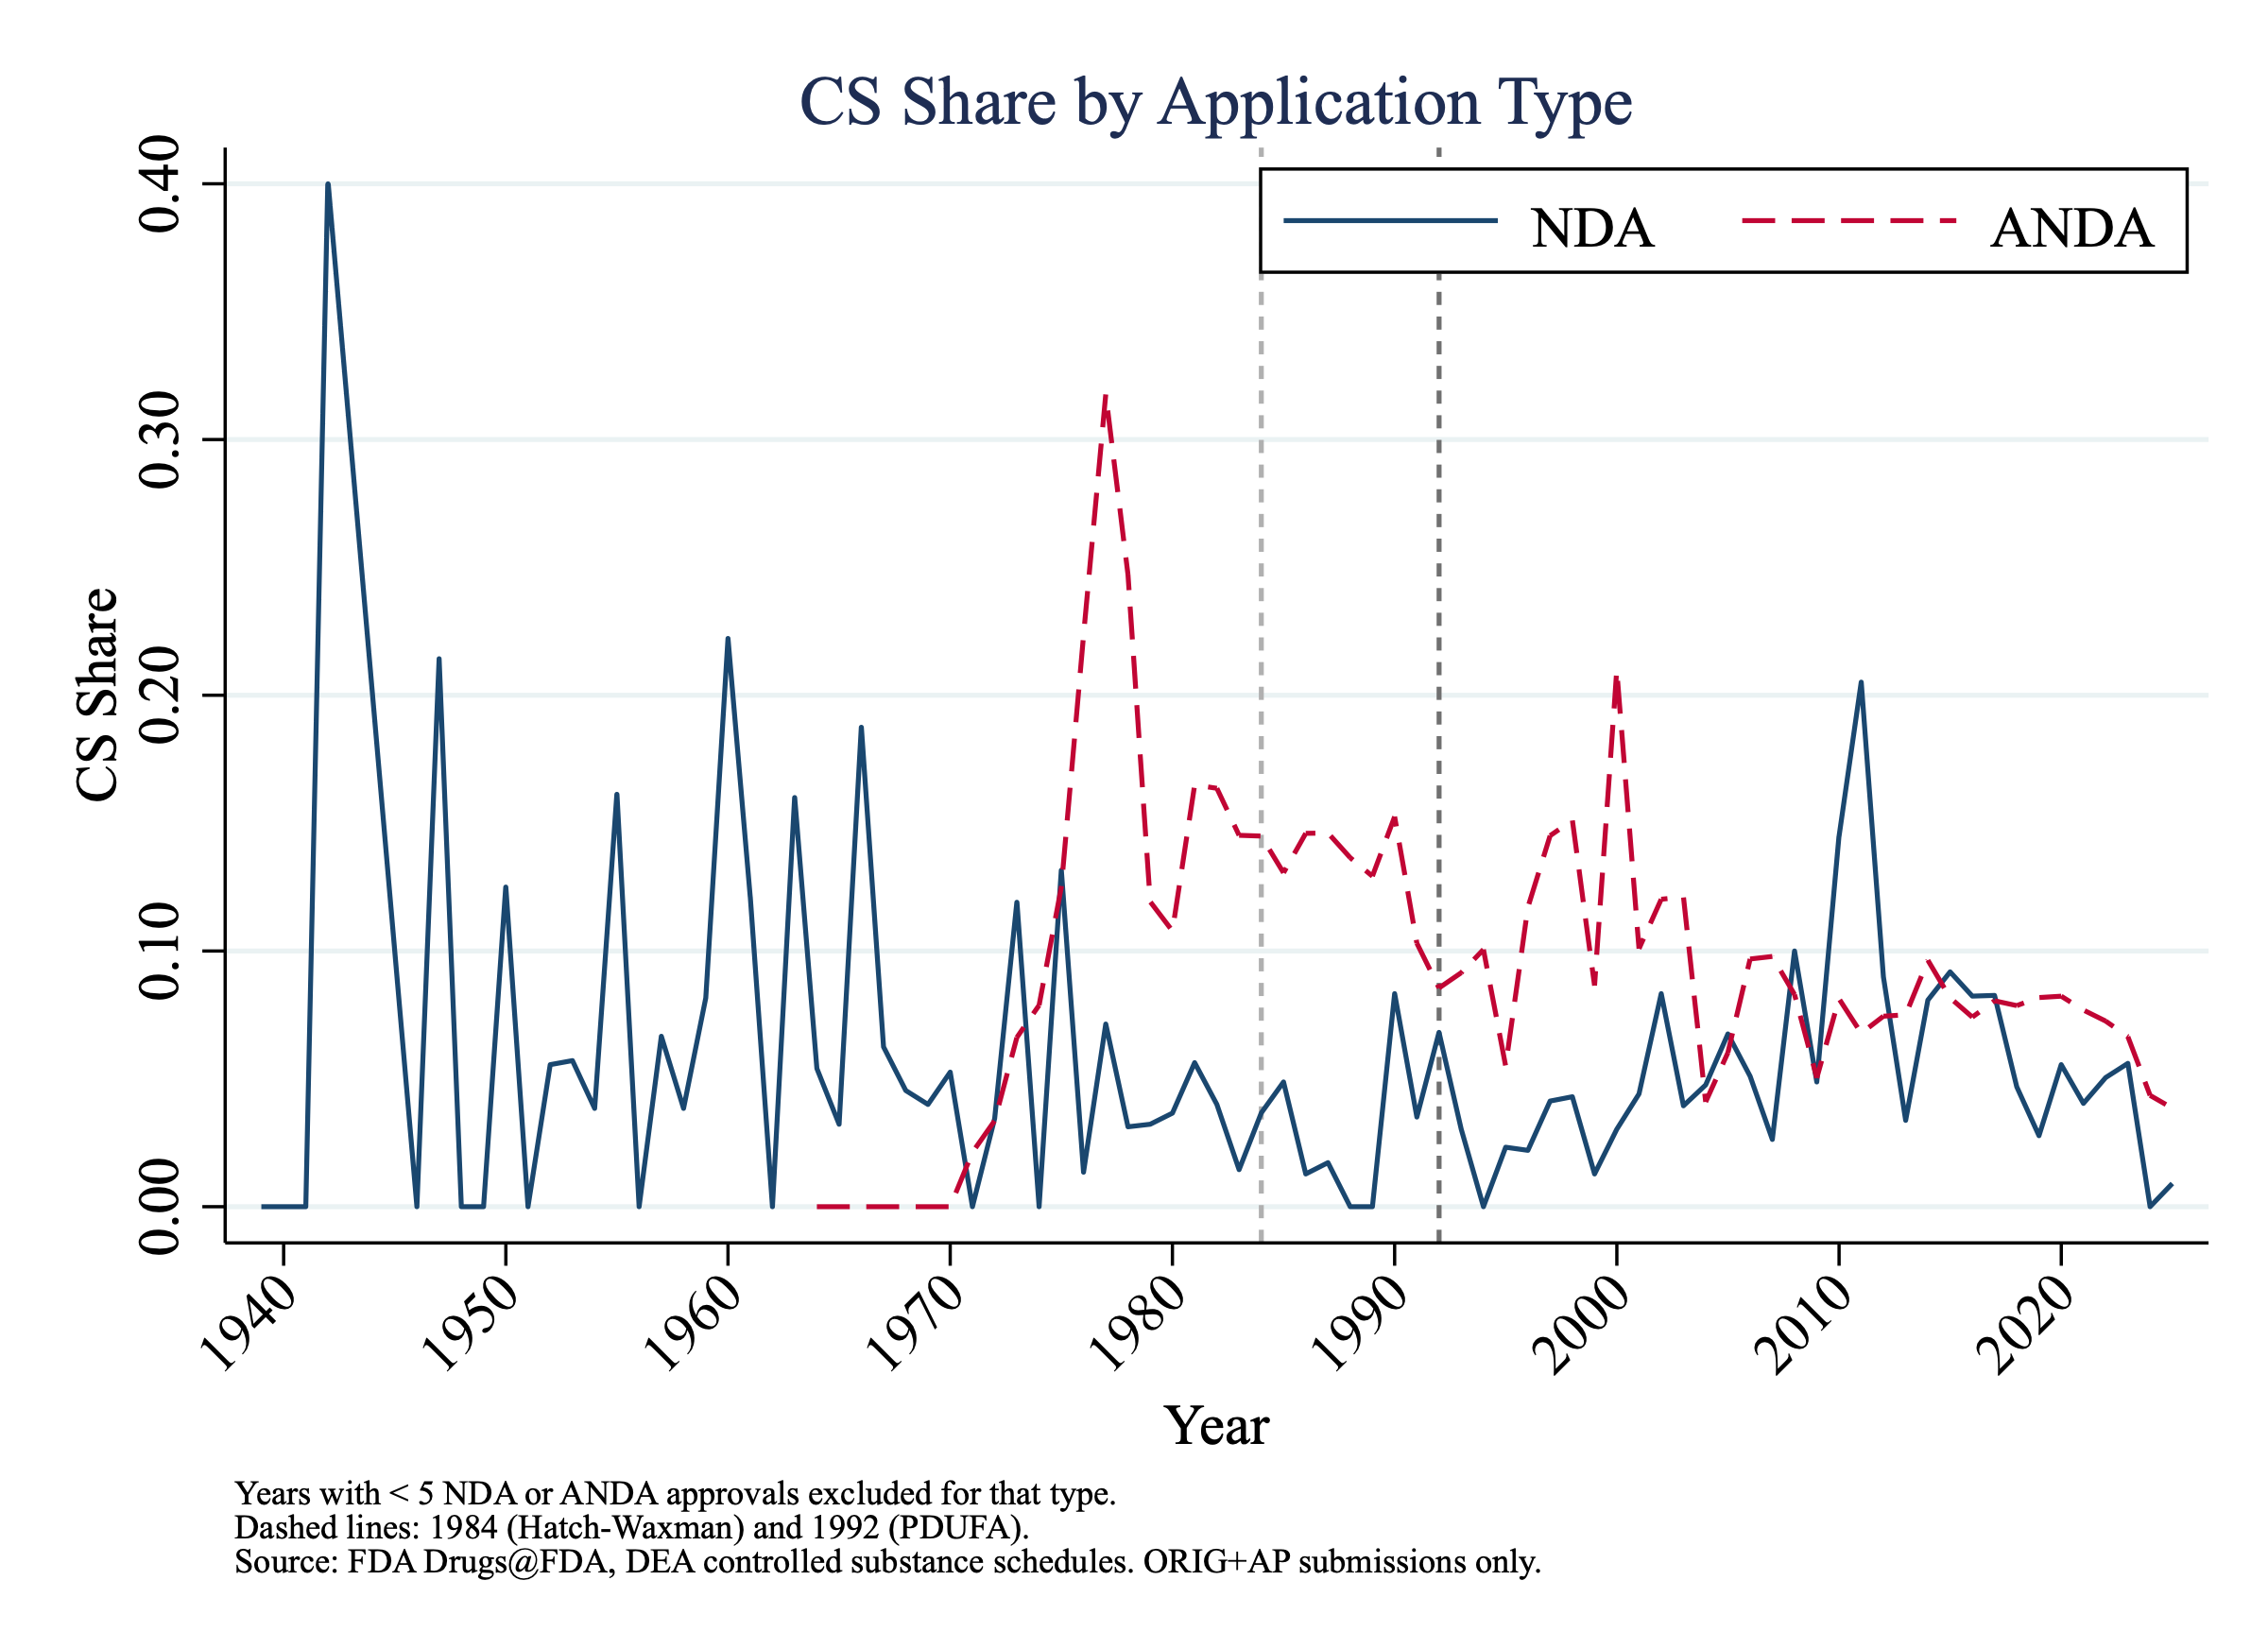
\includegraphics[width=0.92\textwidth]{../output/figures/stata/fig_cs_share_by_appltype.png}
\caption{Annual CS share by application type (NDA vs.\ ANDA), 1939--2025. Years with fewer than five NDA or ANDA approvals are excluded. Dashed lines as in Figure~\ref{fig:cs_share_full}.}
\label{fig:cs_share_by_type}
\end{figure}

\subsection{PDUFA Event Study: Full Sample}
\label{sec:results_pdufa_full}

Figure~\ref{fig:event_study_full} reports event-study point estimates and 95\% confidence intervals from the share-based ITS specification of equation~\ref{eq:its}, with event time measured in years relative to PDUFA (1992). Pre-policy estimates ($\tau < 0$) are clustered near zero, consistent with the parallel-trends assumption over the pre-PDUFA window. Post-policy estimates ($\tau > 0$) move modestly above and below zero with no clear level shift or trend break at $\tau = 0$. The confidence intervals are wide --- a feature of any single national time series --- but they are tight enough to bound the immediate post-1992 deviation from the pre-trend within roughly a percentage-point band.

\begin{figure}[htbp]
\centering
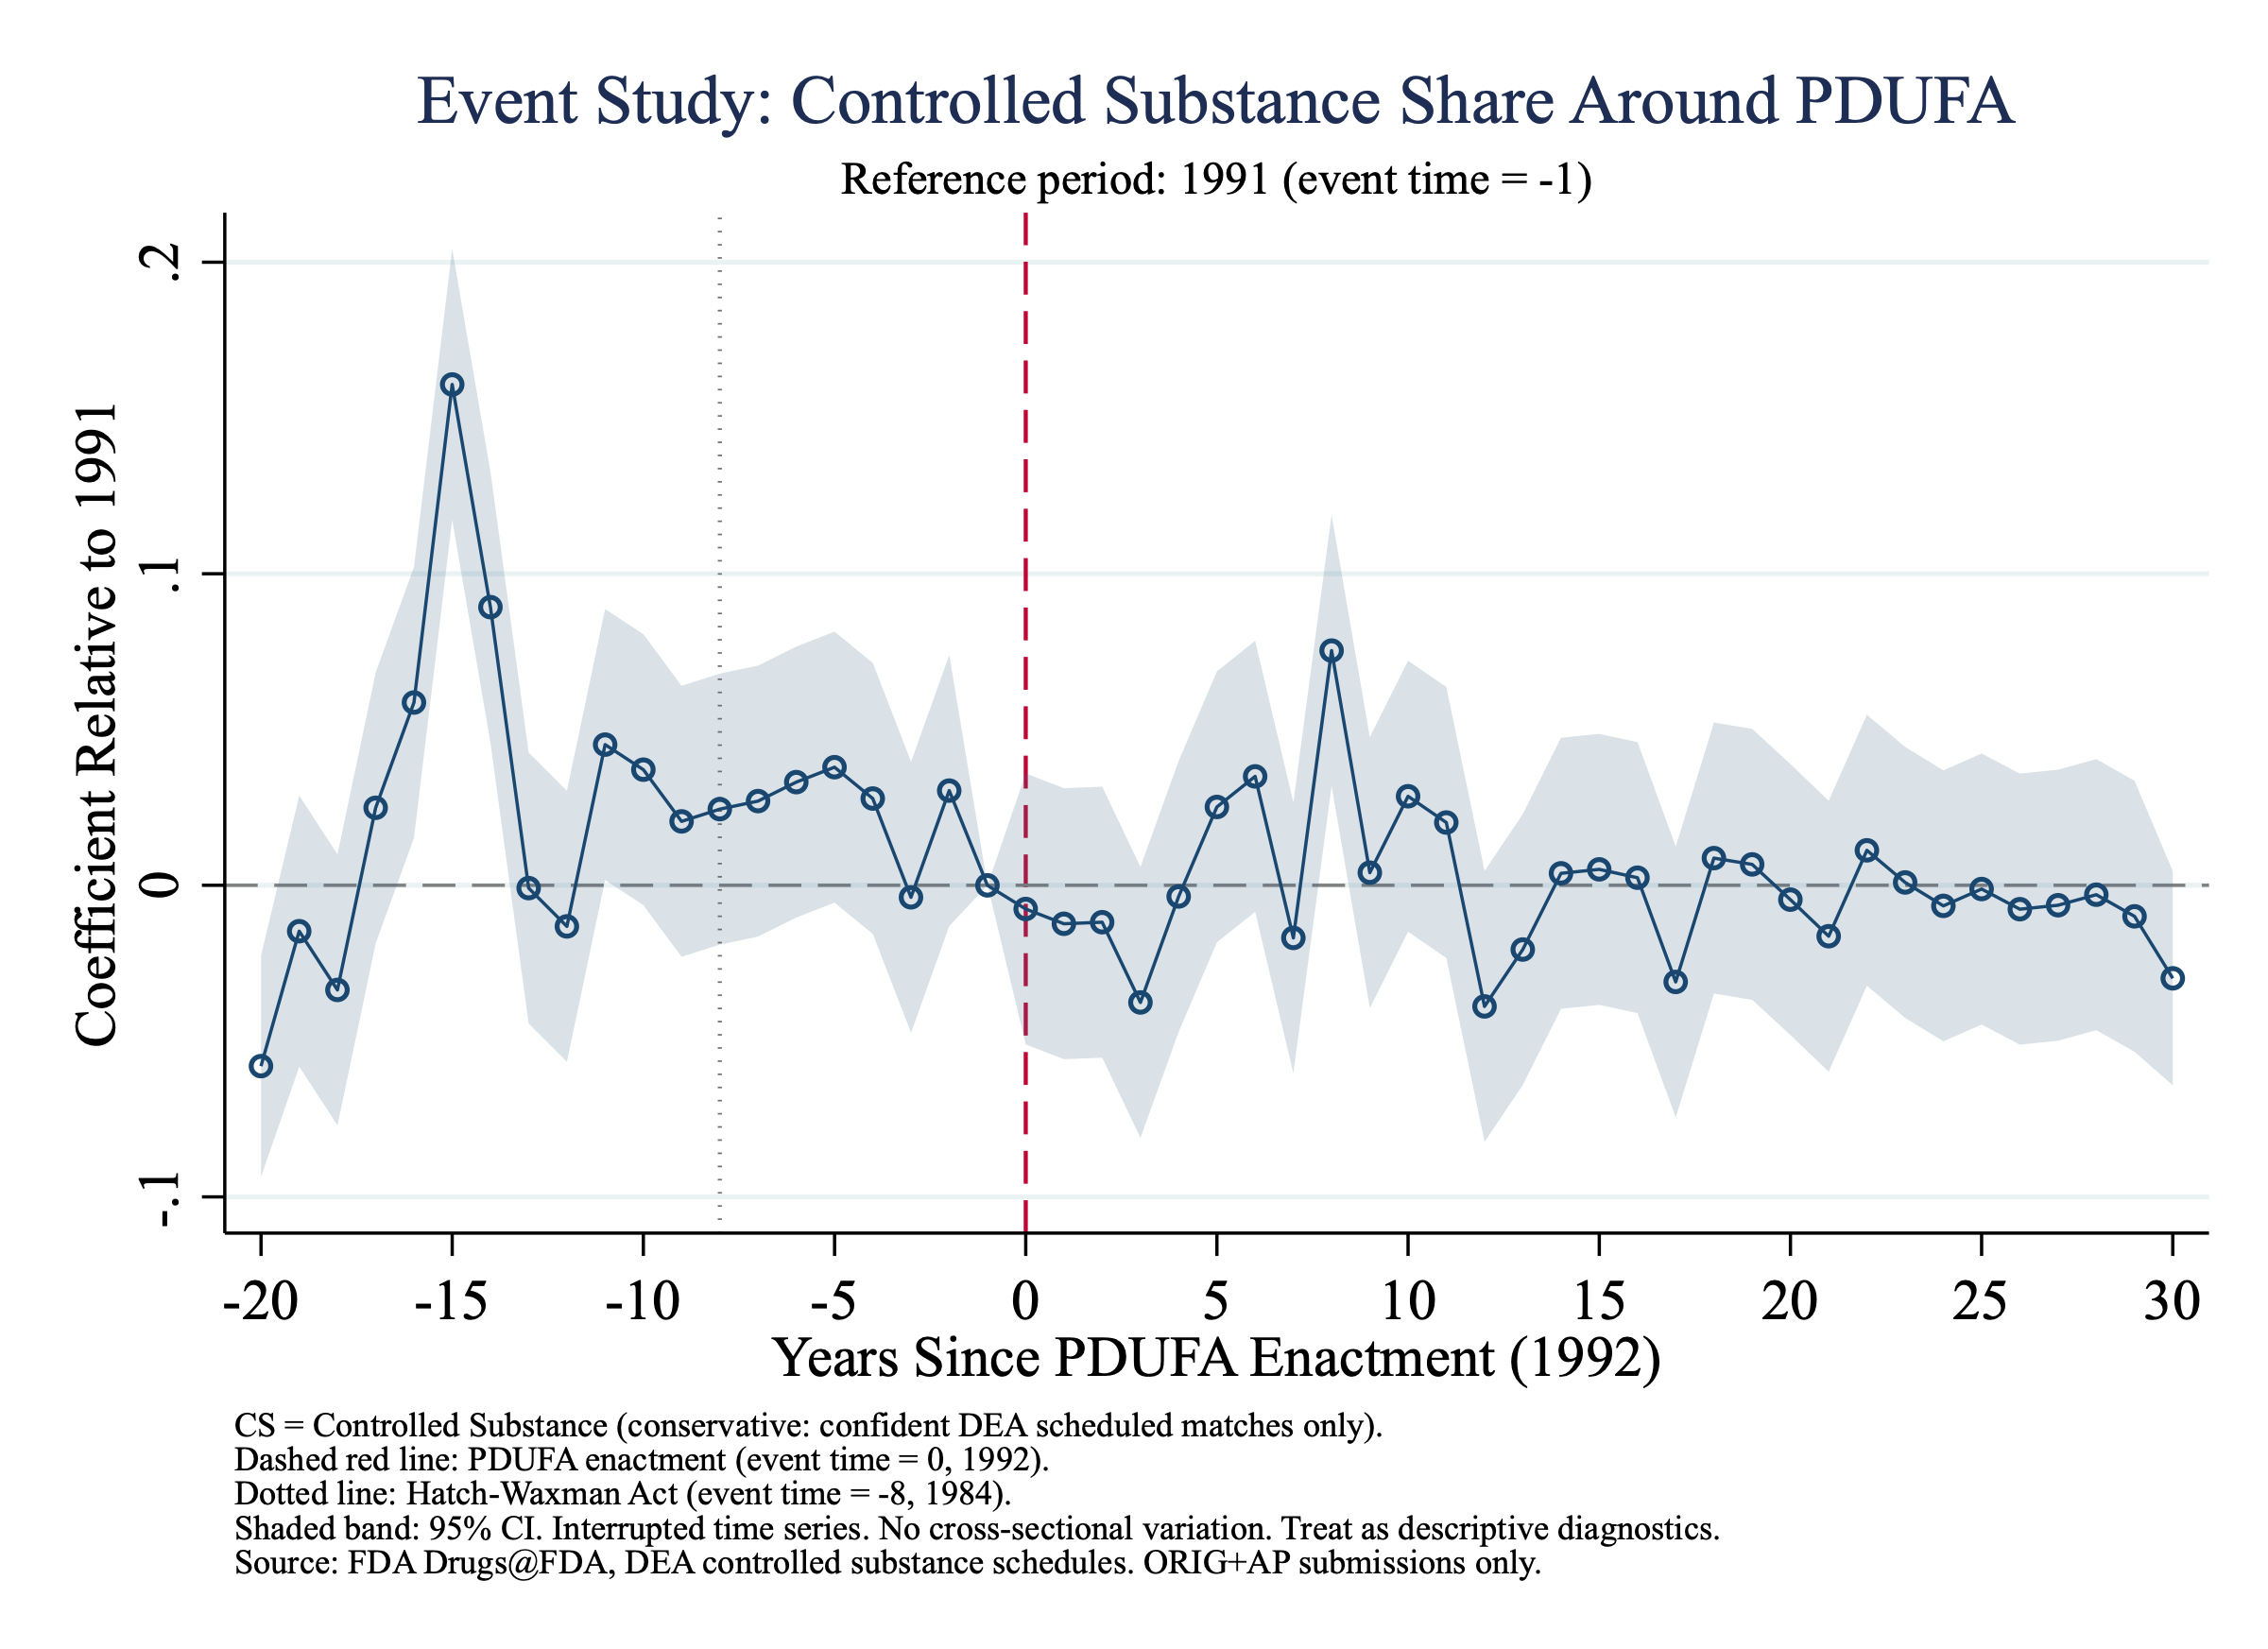
\includegraphics[width=0.92\textwidth]{../output/figures/stata/event_study_cs_share.png}
\caption{PDUFA event study: ITS coefficients on CS share. Event time 0 = 1992 (PDUFA enactment). Reference period: $\tau = -1$ (1991). End-caps at $[-20, +30]$. 95\% confidence intervals.}
\label{fig:event_study_full}
\end{figure}

\subsection{PDUFA Event Study: NDA-Only Sample}
\label{sec:results_nda}

Figure~\ref{fig:event_study_nda} restricts the event-study to new drug applications. This is the theoretically relevant subsample: PDUFA directly governs NDA review times and does not apply to ANDA submissions. The NDA CS share series is noisier than the pooled series because annual NDA counts are smaller, but the event-study profile reveals a feature that organizes the rest of the analysis: the largest positive deviations from the pre-trend occur around event times 17--19 (calendar years 2009--2011), not at or near $\tau = 0$. A composition response operating through the user-fee channel should appear near the policy date.

\begin{figure}[htbp]
\centering
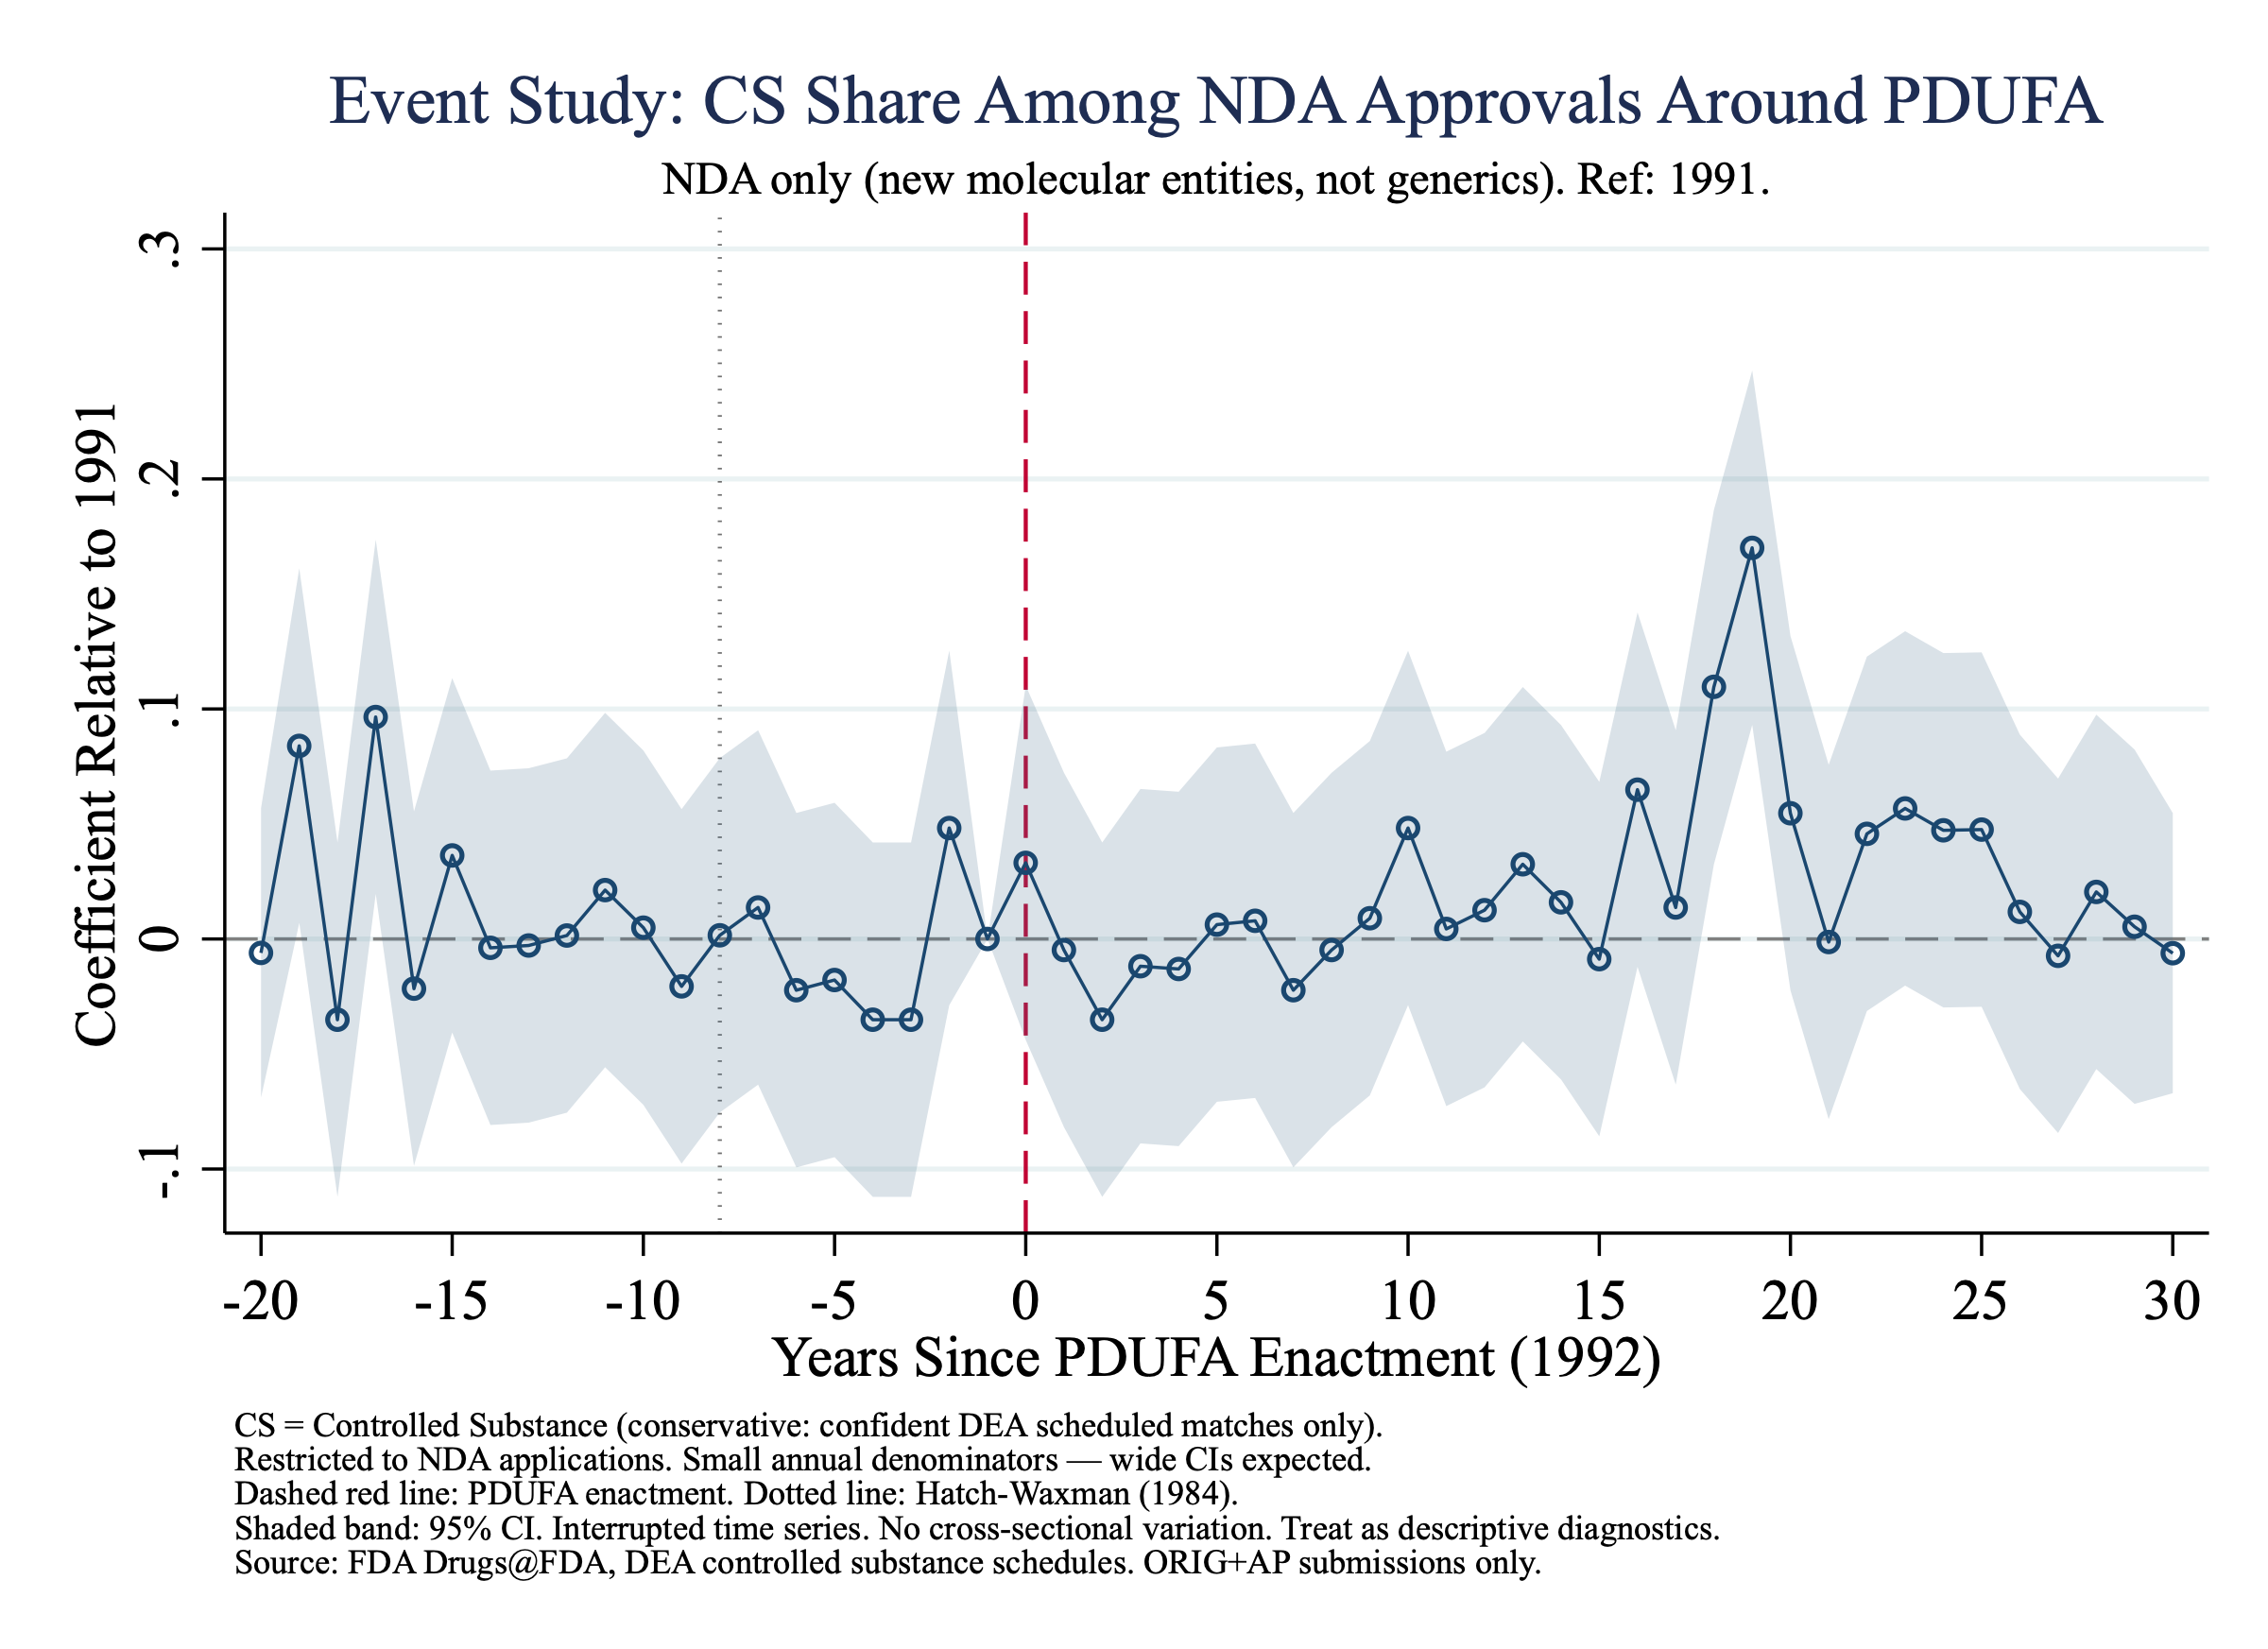
\includegraphics[width=0.92\textwidth]{../output/figures/stata/event_study_cs_share_nda.png}
\caption{PDUFA event study: NDA-only sample. CS share among new drug applications. Event time 0 = 1992. Reference: $\tau = -1$.}
\label{fig:event_study_nda}
\end{figure}

Figure~\ref{fig:nda_share_level} shows the NDA CS share level series with pre-PDUFA and post-PDUFA mean reference lines. The post-PDUFA mean is slightly higher than the pre-PDUFA mean, but the time-series visual makes clear that the difference is concentrated in the 2009--2013 window.

\begin{figure}[htbp]
\centering
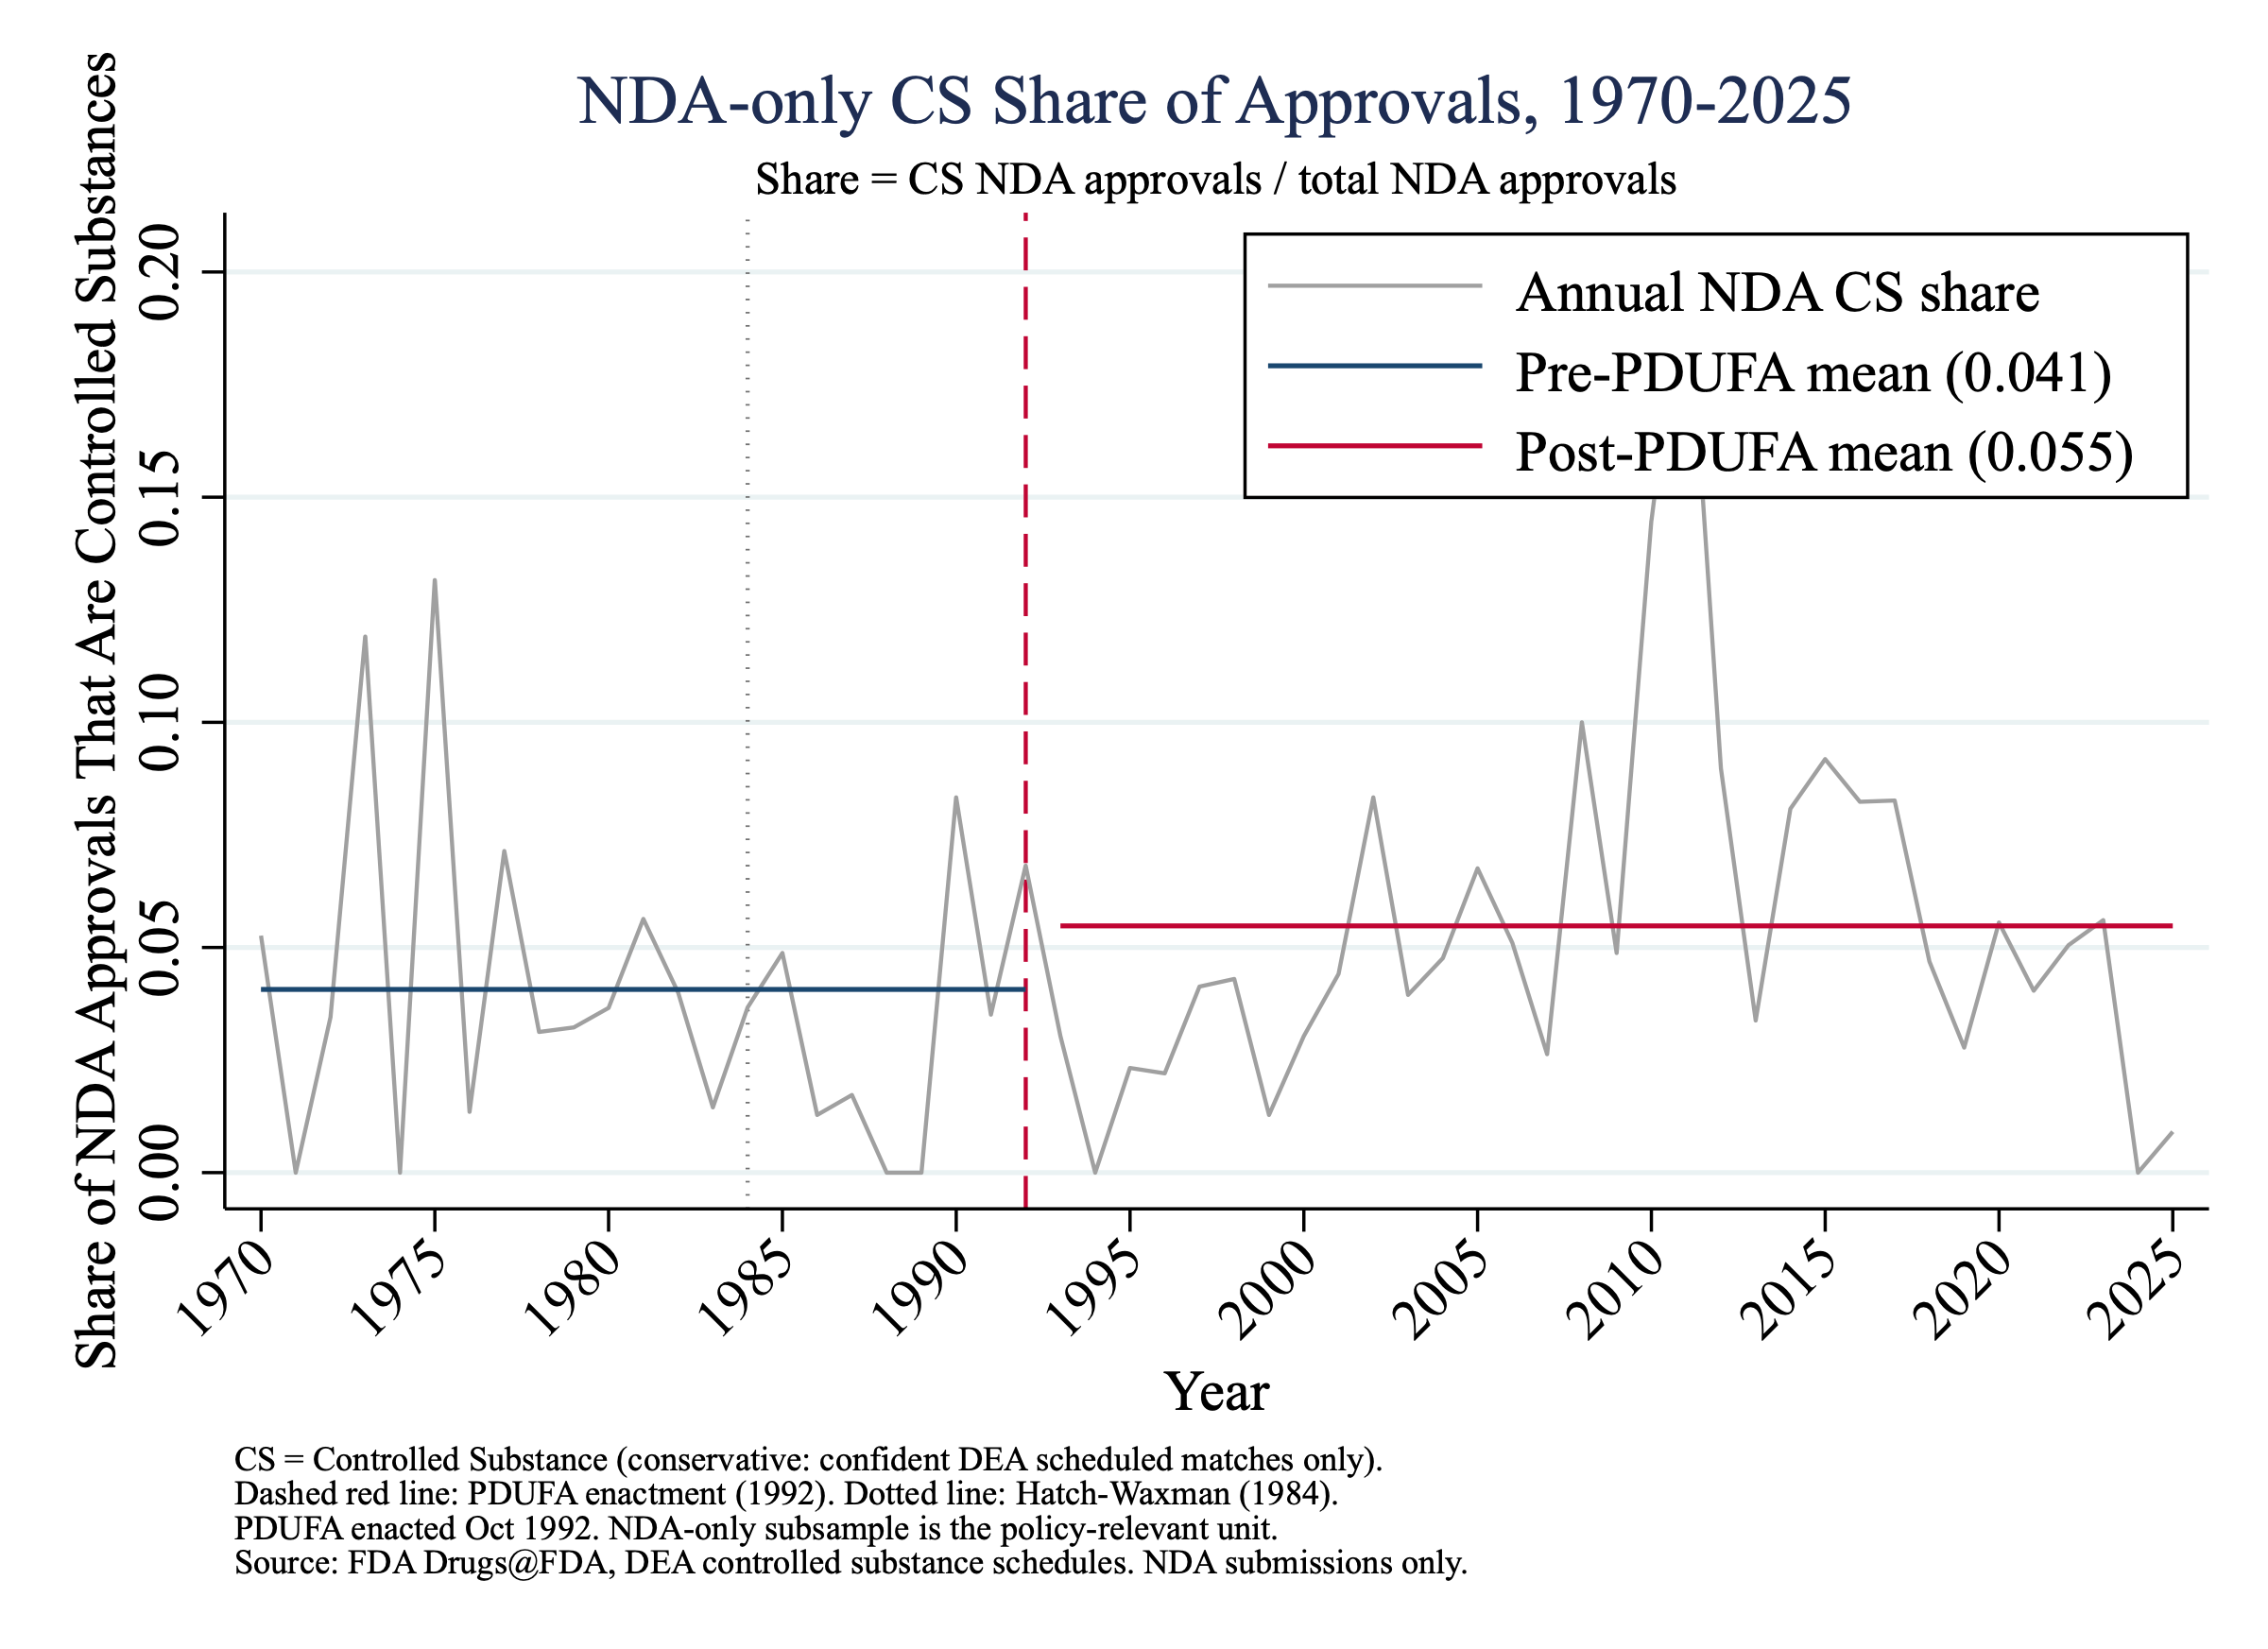
\includegraphics[width=0.92\textwidth]{../output/figures/stata/pdufa_nda_only_share.png}
\caption{NDA controlled-substance share, 1970--2025, with pre/post-PDUFA mean reference lines.}
\label{fig:nda_share_level}
\end{figure}

Table~\ref{tab:pdufa_poisson} reports Poisson rate models for the NDA CS count under three trend specifications. Column~(1) absorbs all year-level variation through year fixed effects. Column~(2) replaces year fixed effects with a single linear time trend. Column~(3) adds group-specific linear trends, allowing the CS and non-CS NDA streams to follow different secular paths. The post-PDUFA incidence-rate ratio in column~(1) is 1.46 ($p = 0.060$), consistent with a 46\% higher CS approval rate post-PDUFA after absorbing year-level variation. Under group-specific trends, the IRR is 1.19 with a 95\% confidence interval of $[0.59, 2.39]$, $p = 0.62$. The point estimate is essentially uninformative: it places the user-fee composition effect on the NDA margin in a band that includes a 41\% reduction and a 139\% increase, with mass concentrated around no effect. The fact that the apparent year-FE elevation is absorbed once group-specific trends accommodate the differential pre/post growth in CS and non-CS NDA streams is the central diagnostic of this section.

\begin{table}[htbp]
\centering
\begin{threeparttable}
\caption{PDUFA NDA-Only Poisson Rate Models: Sensitivity to Trend Controls}
\label{tab:pdufa_poisson}
\small
\begin{tabular}{lccc}
\toprule
 & (1) Year FE & (2) Linear trend & (3) Group trends \\
\midrule
IRR & 1.456 & 1.456 & 1.190 \\
$z$-statistic & 1.879 & 1.832 & 0.490 \\
$p$-value & 0.060 & 0.067 & 0.624 \\
95\% CI & [0.98, 2.16] & [0.97, 2.18] & [0.59, 2.39] \\
\midrule
Observations & \multicolumn{3}{c}{Annual, 1970--2025, NDA only} \\
Exposure & \multicolumn{3}{c}{Total NDA approvals} \\
\bottomrule
\end{tabular}
\begin{tablenotes}
\footnotesize
\item IRR = incidence-rate ratio for the $\text{post\_pdufa} \times \text{is\_cs}$ interaction. Robust standard errors.
\item Column (3) adds separate linear time trends for the CS and non-CS NDA series.
\end{tablenotes}
\end{threeparttable}
\end{table}

Figure~\ref{fig:nda_dd_event} reports the event-study DD coefficients from the NDA-only stacked Poisson specification. The IRR profile sits near unity for all pre-policy event times, consistent with parallel pre-trends. Post-policy IRRs drift upward gradually, peak around event times 17--19 (2009--2011), and subside thereafter. This pattern --- a late-rising post-policy departure that does not appear near the policy date --- is inconsistent with a PDUFA composition effect operating through review-time incentives and is instead consistent with a delayed industry product cycle, as Section~\ref{sec:results_spike} documents at the drug level.

\begin{figure}[htbp]
\centering
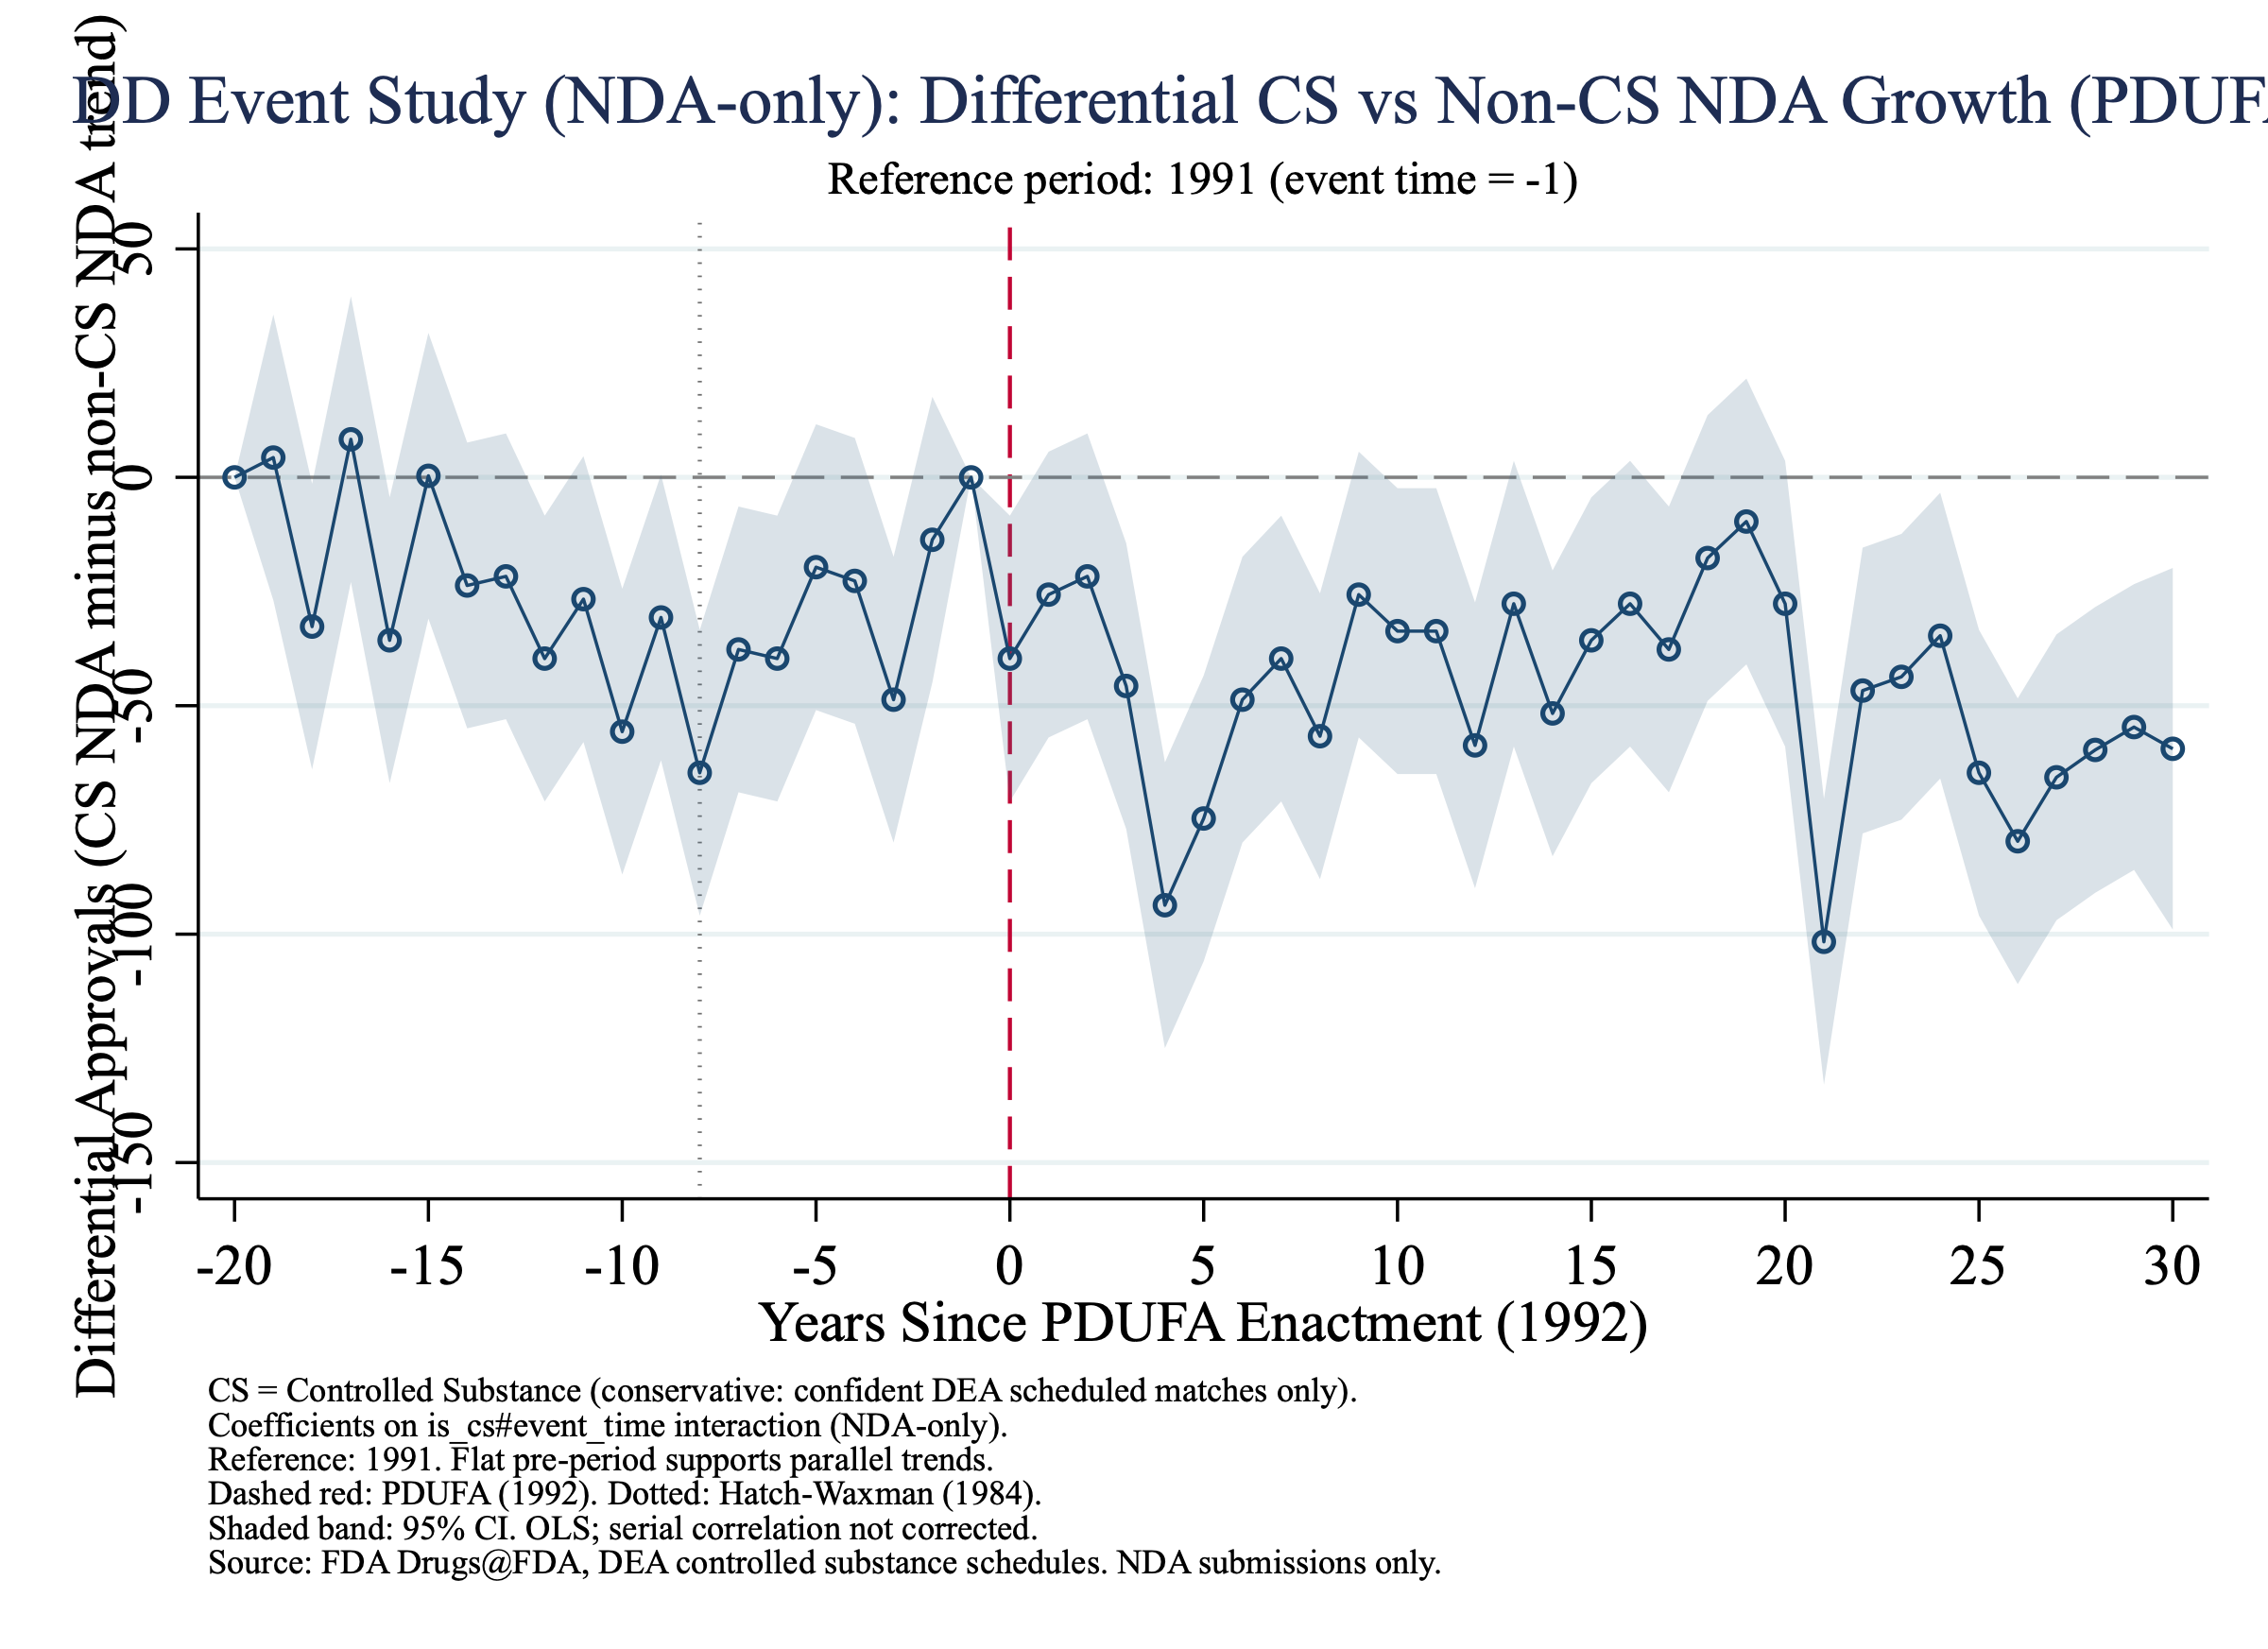
\includegraphics[width=0.92\textwidth]{../output/figures/stata/pdufa_nda_only_dd_event_study.png}
\caption{PDUFA NDA-only stacked Poisson DD event study. IRRs for $\text{CS} \times \mathbf{1}[\tau]$ interactions. Reference: $\tau = -1$ (1991). End-caps at $[-20, +30]$. 95\% CI.}
\label{fig:nda_dd_event}
\end{figure}

\subsection{Rate Versus Count Decomposition}

Figure~\ref{fig:nda_rate_count} decomposes the NDA result into a rate panel and a count panel. Panel~A shows the CS share of NDA approvals; Panel~B shows the absolute counts of CS and non-CS NDA approvals. The two panels are simultaneously consistent: the CS rate rises modestly after 1992 even as the absolute volume of non-CS NDA approvals grows faster in levels. Reading the rate alone could overstate any compositional shift; reading the count alone could understate it. Together they clarify that the apparent post-PDUFA NDA elevation reflects a small numerator increase concentrated in a narrow window, not a sustained reorientation of the NDA portfolio.

\begin{figure}[htbp]
\centering
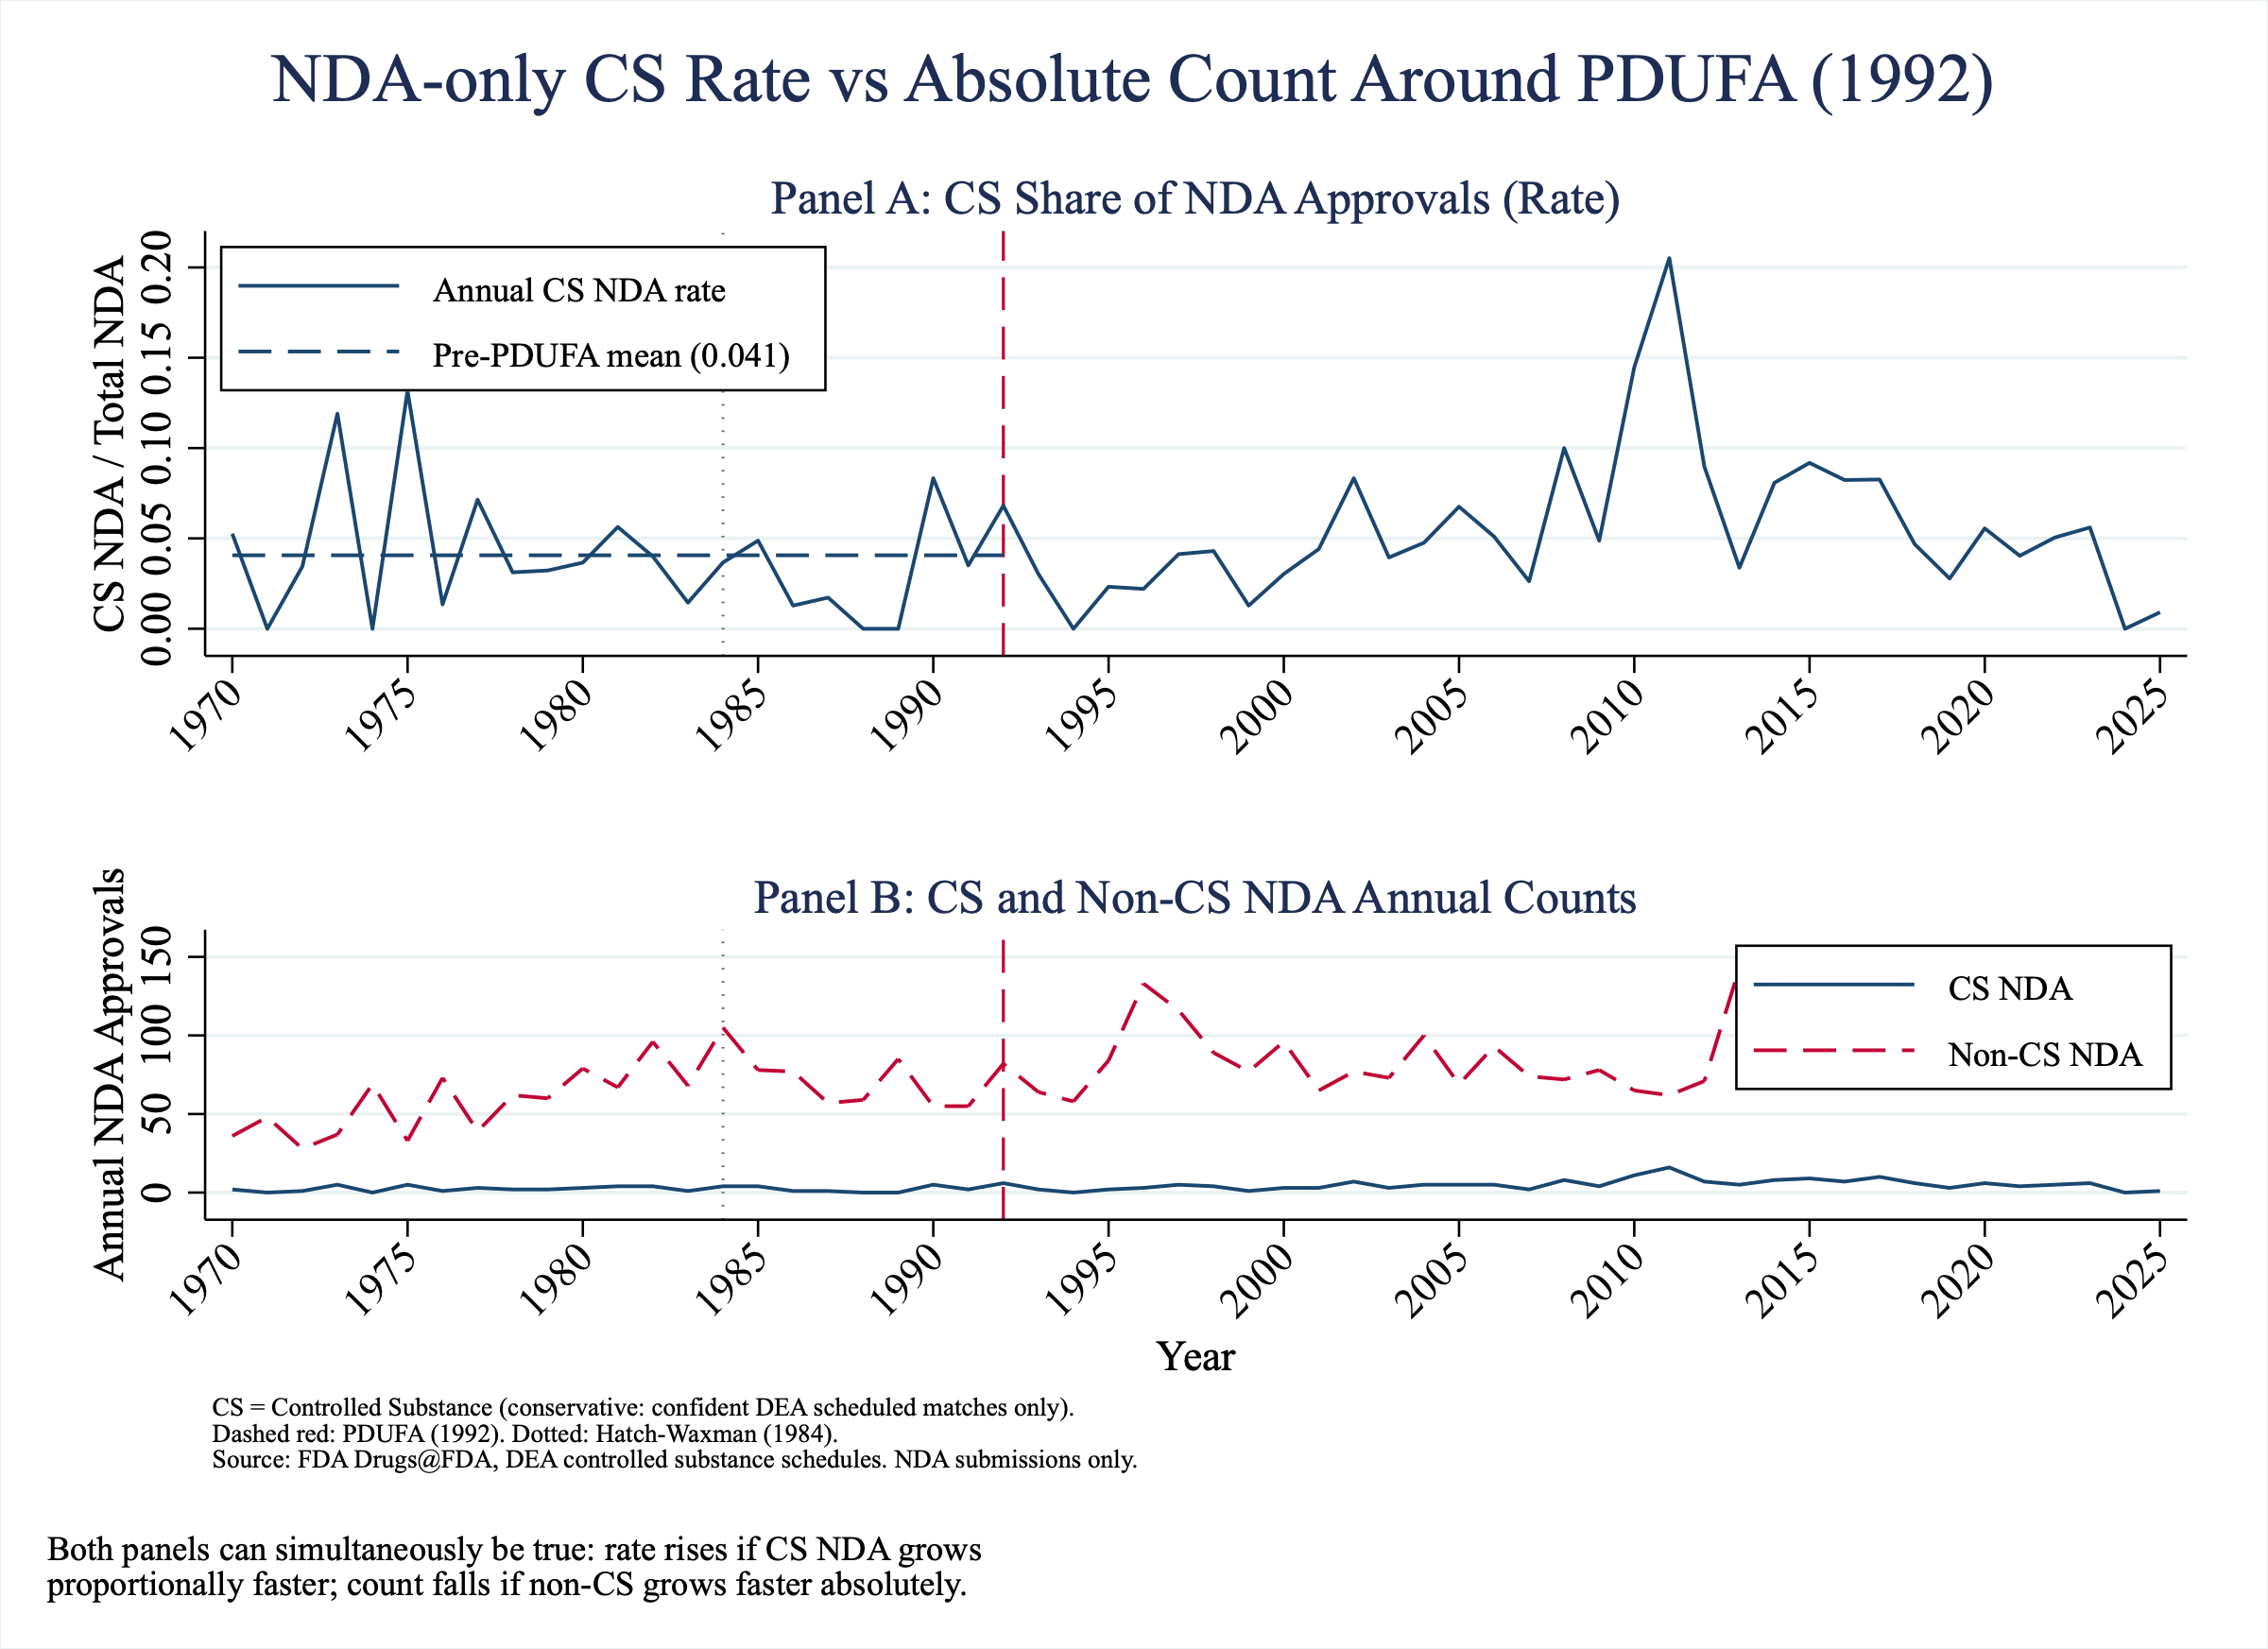
\includegraphics[width=0.92\textwidth]{../output/figures/stata/pdufa_nda_rate_vs_count.png}
\caption{NDA CS approvals: rate (Panel A) and absolute count (Panel B). Panel A shows CS share among NDA approvals with pre-PDUFA mean reference line. Panel B shows annual CS NDA count vs.\ non-CS NDA count.}
\label{fig:nda_rate_count}
\end{figure}

\subsection{The 2009--2013 CS NDA Spike}
\label{sec:results_spike}

The event-study and time-series evidence point to a cluster of Schedule~II NDA approvals concentrated in 2009--2013. Table~\ref{tab:spike_drugs} lists representative CS NDA approvals from this window, identifying the brand name, active ingredient, sponsor, and DEA schedule for each drug. Four features stand out. First, 43 CS NDAs were approved in this five-year window, compared with an average of roughly six to eight per year in the preceding decade. Second, 2011 alone accounts for 16 CS NDA approvals --- by far the largest single-year count in the sample. Third, 25 of the 43 approvals (58\%) are Schedule~II, the most restrictive category for drugs with accepted medical use. Fourth, the drug list maps closely onto the well-documented wave of branded extended-release and abuse-deterrent opioid formulations that characterized the late-2000s pharmaceutical market: the reformulated OxyContin (Purdue Pharma, 2010), Exalgo (Specgx, 2010), Embeda (Alpharma, 2009), Suboxone (Indivior, 2010), Zohydro ER (Zogenix, 2012), and related products.

\begin{table}[htbp]
\centering
\begin{threeparttable}
\caption{CS NDA Approvals, 2009--2013 (Selected)}
\label{tab:spike_drugs}
\small
\begin{tabular}{llllr}
\toprule
Year & Brand Name & Active Ingredient & Sponsor & Sched. \\
\midrule
2009 & ONSOLIS & Fentanyl citrate & ADALVO & II \\
2009 & EMBEDA & Morphine sulfate; naltrexone & ALPHARMA & II \\
2009 & CODEINE SULFATE & Codeine sulfate & HIKMA & II \\
2009 & EDLUAR & Zolpidem tartrate & VIATRIS & IV \\
2010 & EXALGO & Hydromorphone HCl & SPECGX LLC & II \\
2010 & OXYCONTIN & Oxycodone HCl & PURDUE PHARMA & II \\
2010 & SUBOXONE & Buprenorphine; naloxone & INDIVIOR & III \\
2010 & BUTRANS & Buprenorphine & PURDUE PHARMA & III \\
2010 & AXIRON & Testosterone & ELI LILLY & III \\
2010 & LYRICA & Pregabalin & UPJOHN & V \\
2011 & ANDROGEL & Testosterone & BESINS HLTHCARE & III \\
2011 & INTERMEZZO & Zolpidem tartrate & PURDUE PHARMA & IV \\
2012 & ZOHYDRO ER & Hydrocodone bitartrate & ZOGENIX & II \\
\midrule
\multicolumn{5}{l}{\textit{Full 2009--2013 window: 43 CS NDAs; 25 Schedule~II (58\%); 2011 peak: 16 approvals.}} \\
\bottomrule
\end{tabular}
\begin{tablenotes}
\footnotesize
\item Selected rows for illustration. Full list in \texttt{output/tables/stata/cs\_nda\_2009\_2013\_drugs.csv}.
\item OxyContin (2010) is the reformulated abuse-deterrent NDA (NDA 022272), not the original 1995 approval.
\end{tablenotes}
\end{threeparttable}
\end{table}

The timing of these approvals --- seventeen to twenty-one years after PDUFA enactment --- and their close correspondence to a documented pharmaceutical product cycle make them difficult to attribute to user-fee incentives. Once the late-2000s opioid wave is allowed to load onto its own group-specific trend in column~(3) of Table~\ref{tab:pdufa_poisson}, the post-PDUFA IRR moves toward unity and the wide confidence interval $[0.59, 2.39]$ obtains.

\subsection{GDUFA Event Study: ANDA-Only}
\label{sec:results_gdufa}

Figure~\ref{fig:gdufa_event} reports the GDUFA event-study DD for the ANDA-only sample. Pre-policy event-time coefficients sit near zero, supporting the parallel-trends assumption over the 2002--2012 pre-GDUFA window. Post-policy IRRs decline through the 2015--2025 performance-goal era. The stacked Poisson DD specification (Table~\ref{tab:gdufa_results}) yields a year-FE IRR of $0.668$ ($p < 0.001$, 95\% CI $[0.55, 0.81]$), implying that the CS share of ANDA approvals fell by approximately one-third relative to the non-CS share after 2015. The level result is robust to a single linear time trend ($p = 0.008$).

\begin{figure}[htbp]
\centering
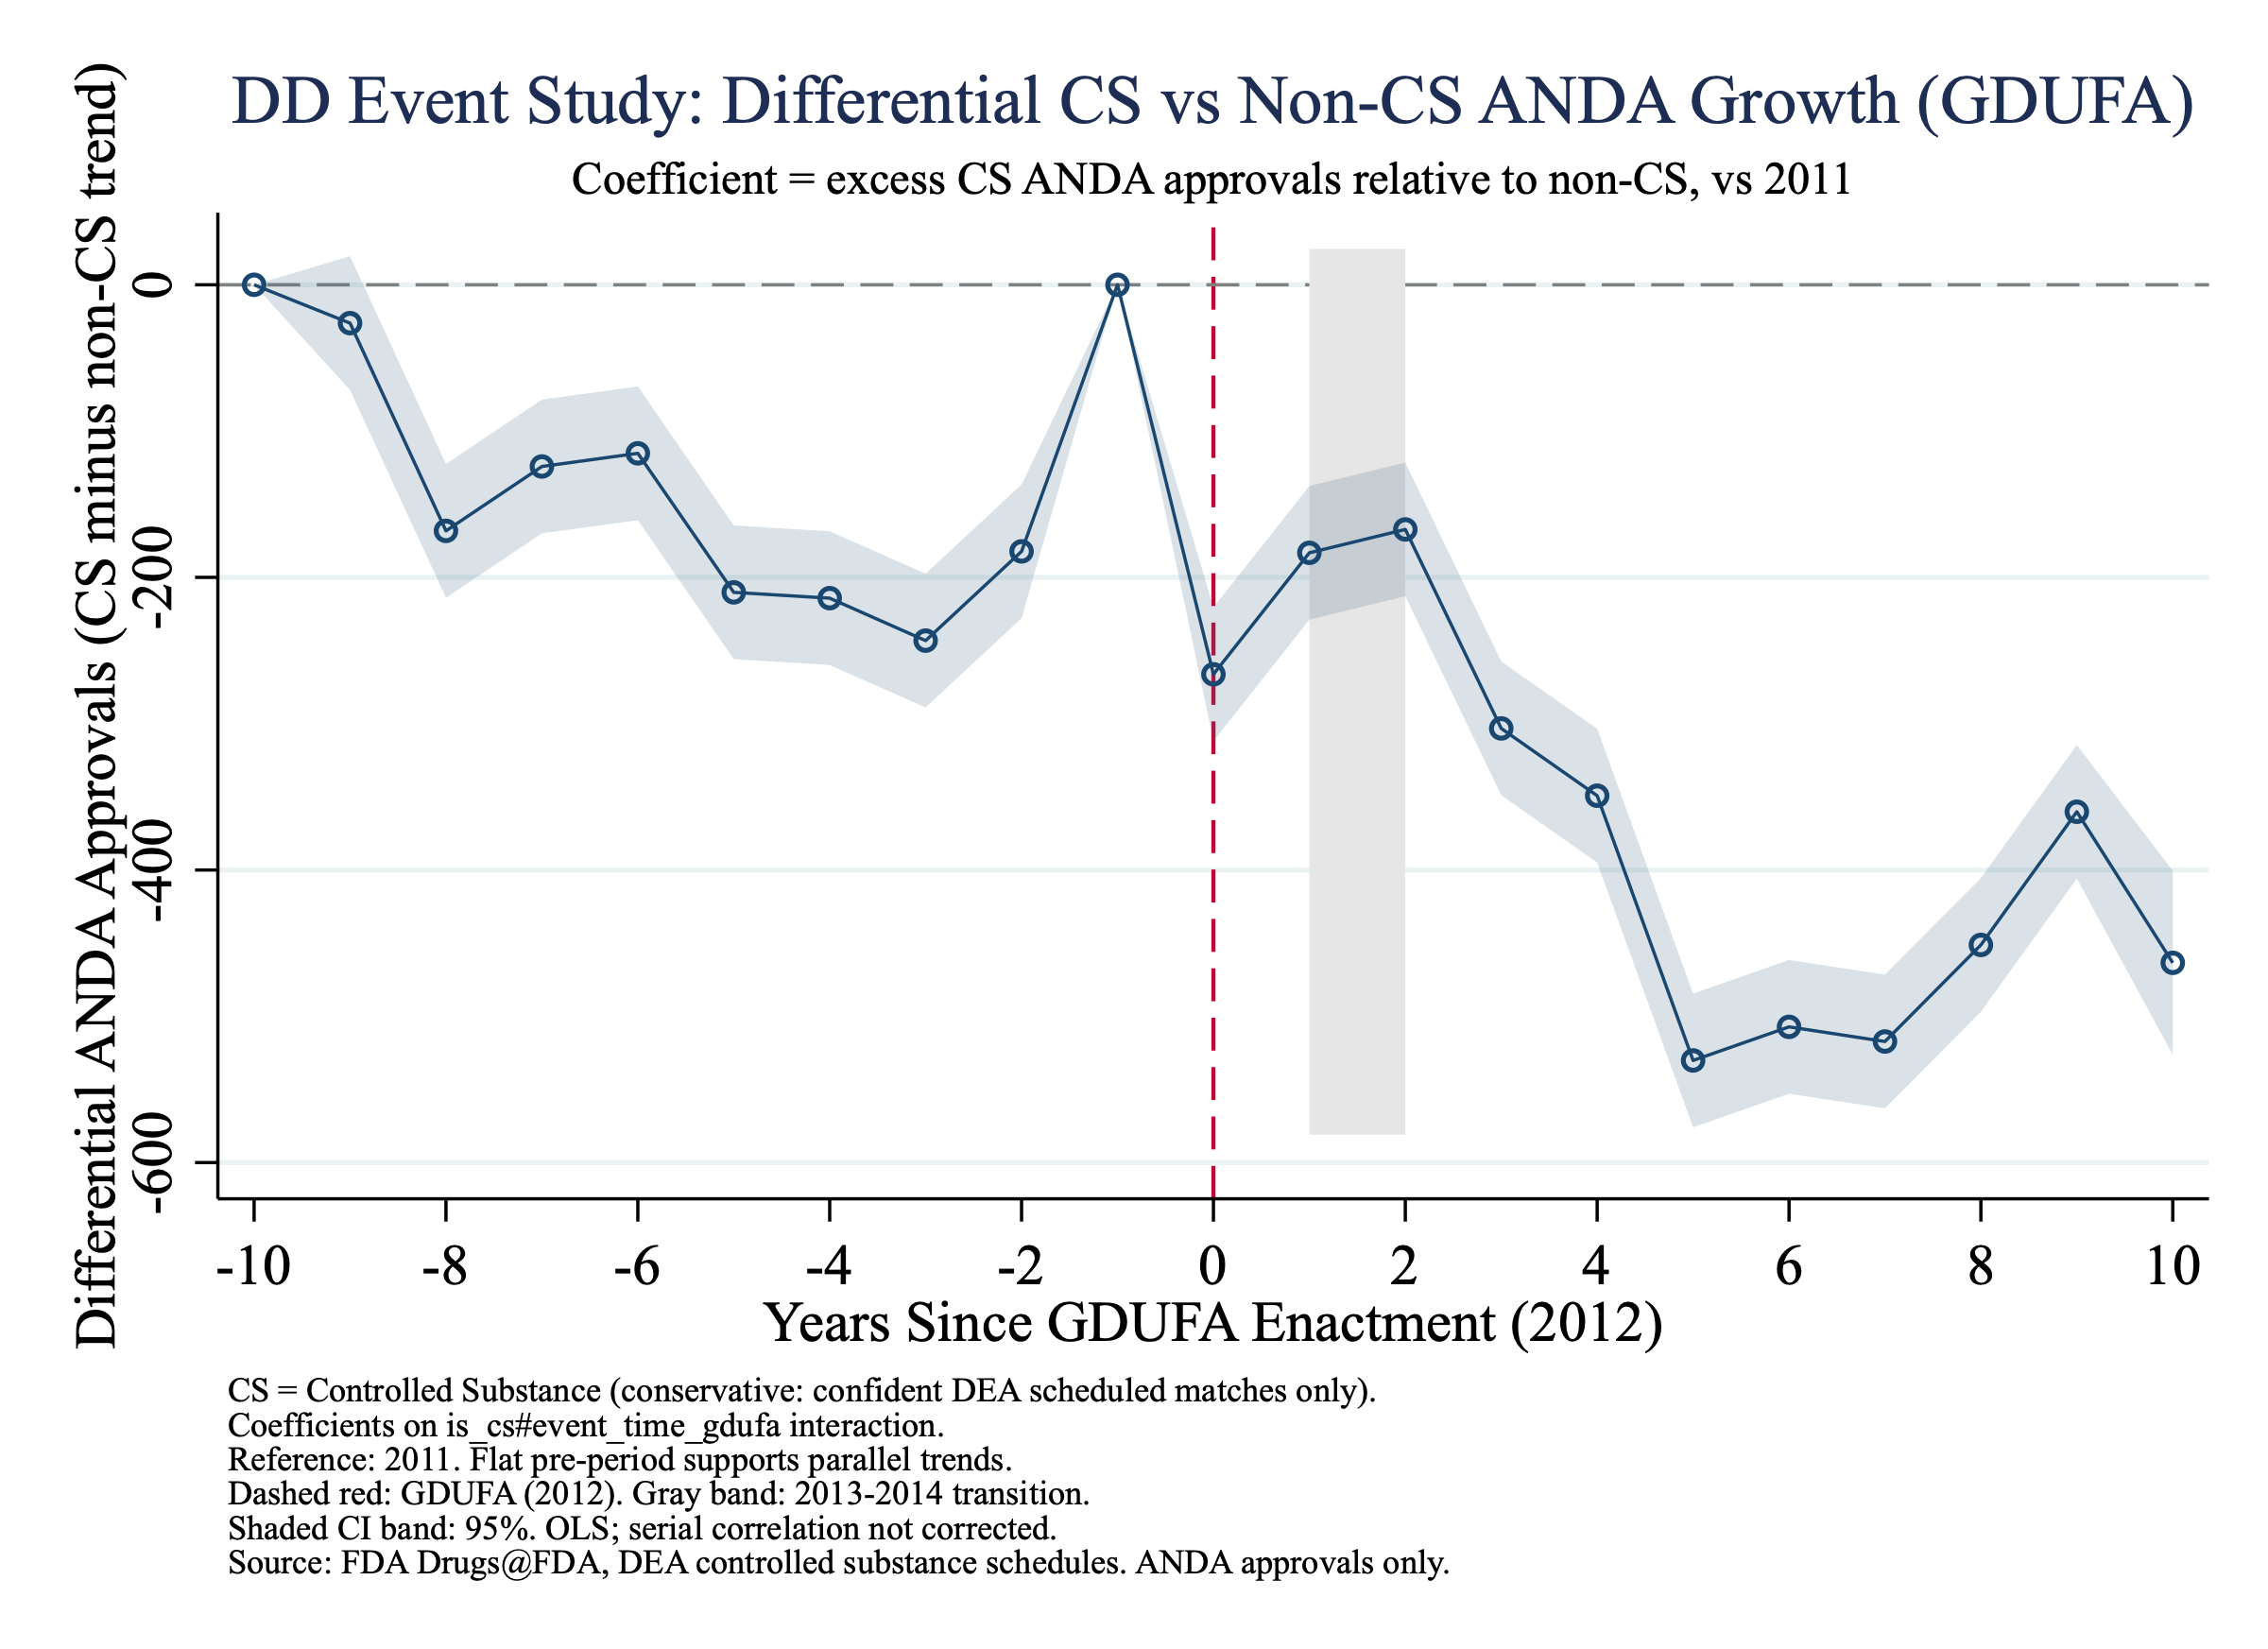
\includegraphics[width=0.92\textwidth]{../output/figures/stata/gdufa_dd_event_study.png}
\caption{GDUFA ANDA-only stacked Poisson DD event study. IRRs for $\text{CS} \times \mathbf{1}[\tau]$ interactions. Reference: $\tau = -1$ (2011). End-caps at $[-10, +10]$. Transition years 2013--2014 excluded. 95\% CI.}
\label{fig:gdufa_event}
\end{figure}

The robustness story changes once group-specific linear trends are added. Allowing the CS-ANDA and non-CS-ANDA series to follow their own pre-period trajectories yields an IRR of $1.38$ with a 95\% confidence interval of $[0.86, 2.21]$ and $p = 0.18$ --- a point estimate that not only fails to attain conventional significance but also flips sign relative to the year-FE specification. The level decline observed in the year-FE specification is absorbed once the analysis allows for the steady pre-policy decline in the CS share of ANDA approvals that began well before GDUFA. Read together, these results argue for the same null interpretation as the PDUFA evidence: the user-fee composition effect on the ANDA controlled-substance margin is not separately identified from a longer-running secular trend.

Figure~\ref{fig:gdufa_rate_count} decomposes the GDUFA result into rate (Panel A) and count (Panel B). Panel A shows the ANDA CS share declining from a pre-GDUFA mean of 10.8\% to a post-GDUFA mean of approximately 7.1\%. Panel B shows that both the CS ANDA count and the non-CS ANDA count declined in absolute terms after GDUFA, with the CS count falling proportionally more steeply. The decomposition makes clear that the year-FE result is a relative one --- both series fall, and the CS series falls faster --- which is consistent with the pre-existing trend interpretation rather than with a post-GDUFA structural break.

\begin{figure}[htbp]
\centering
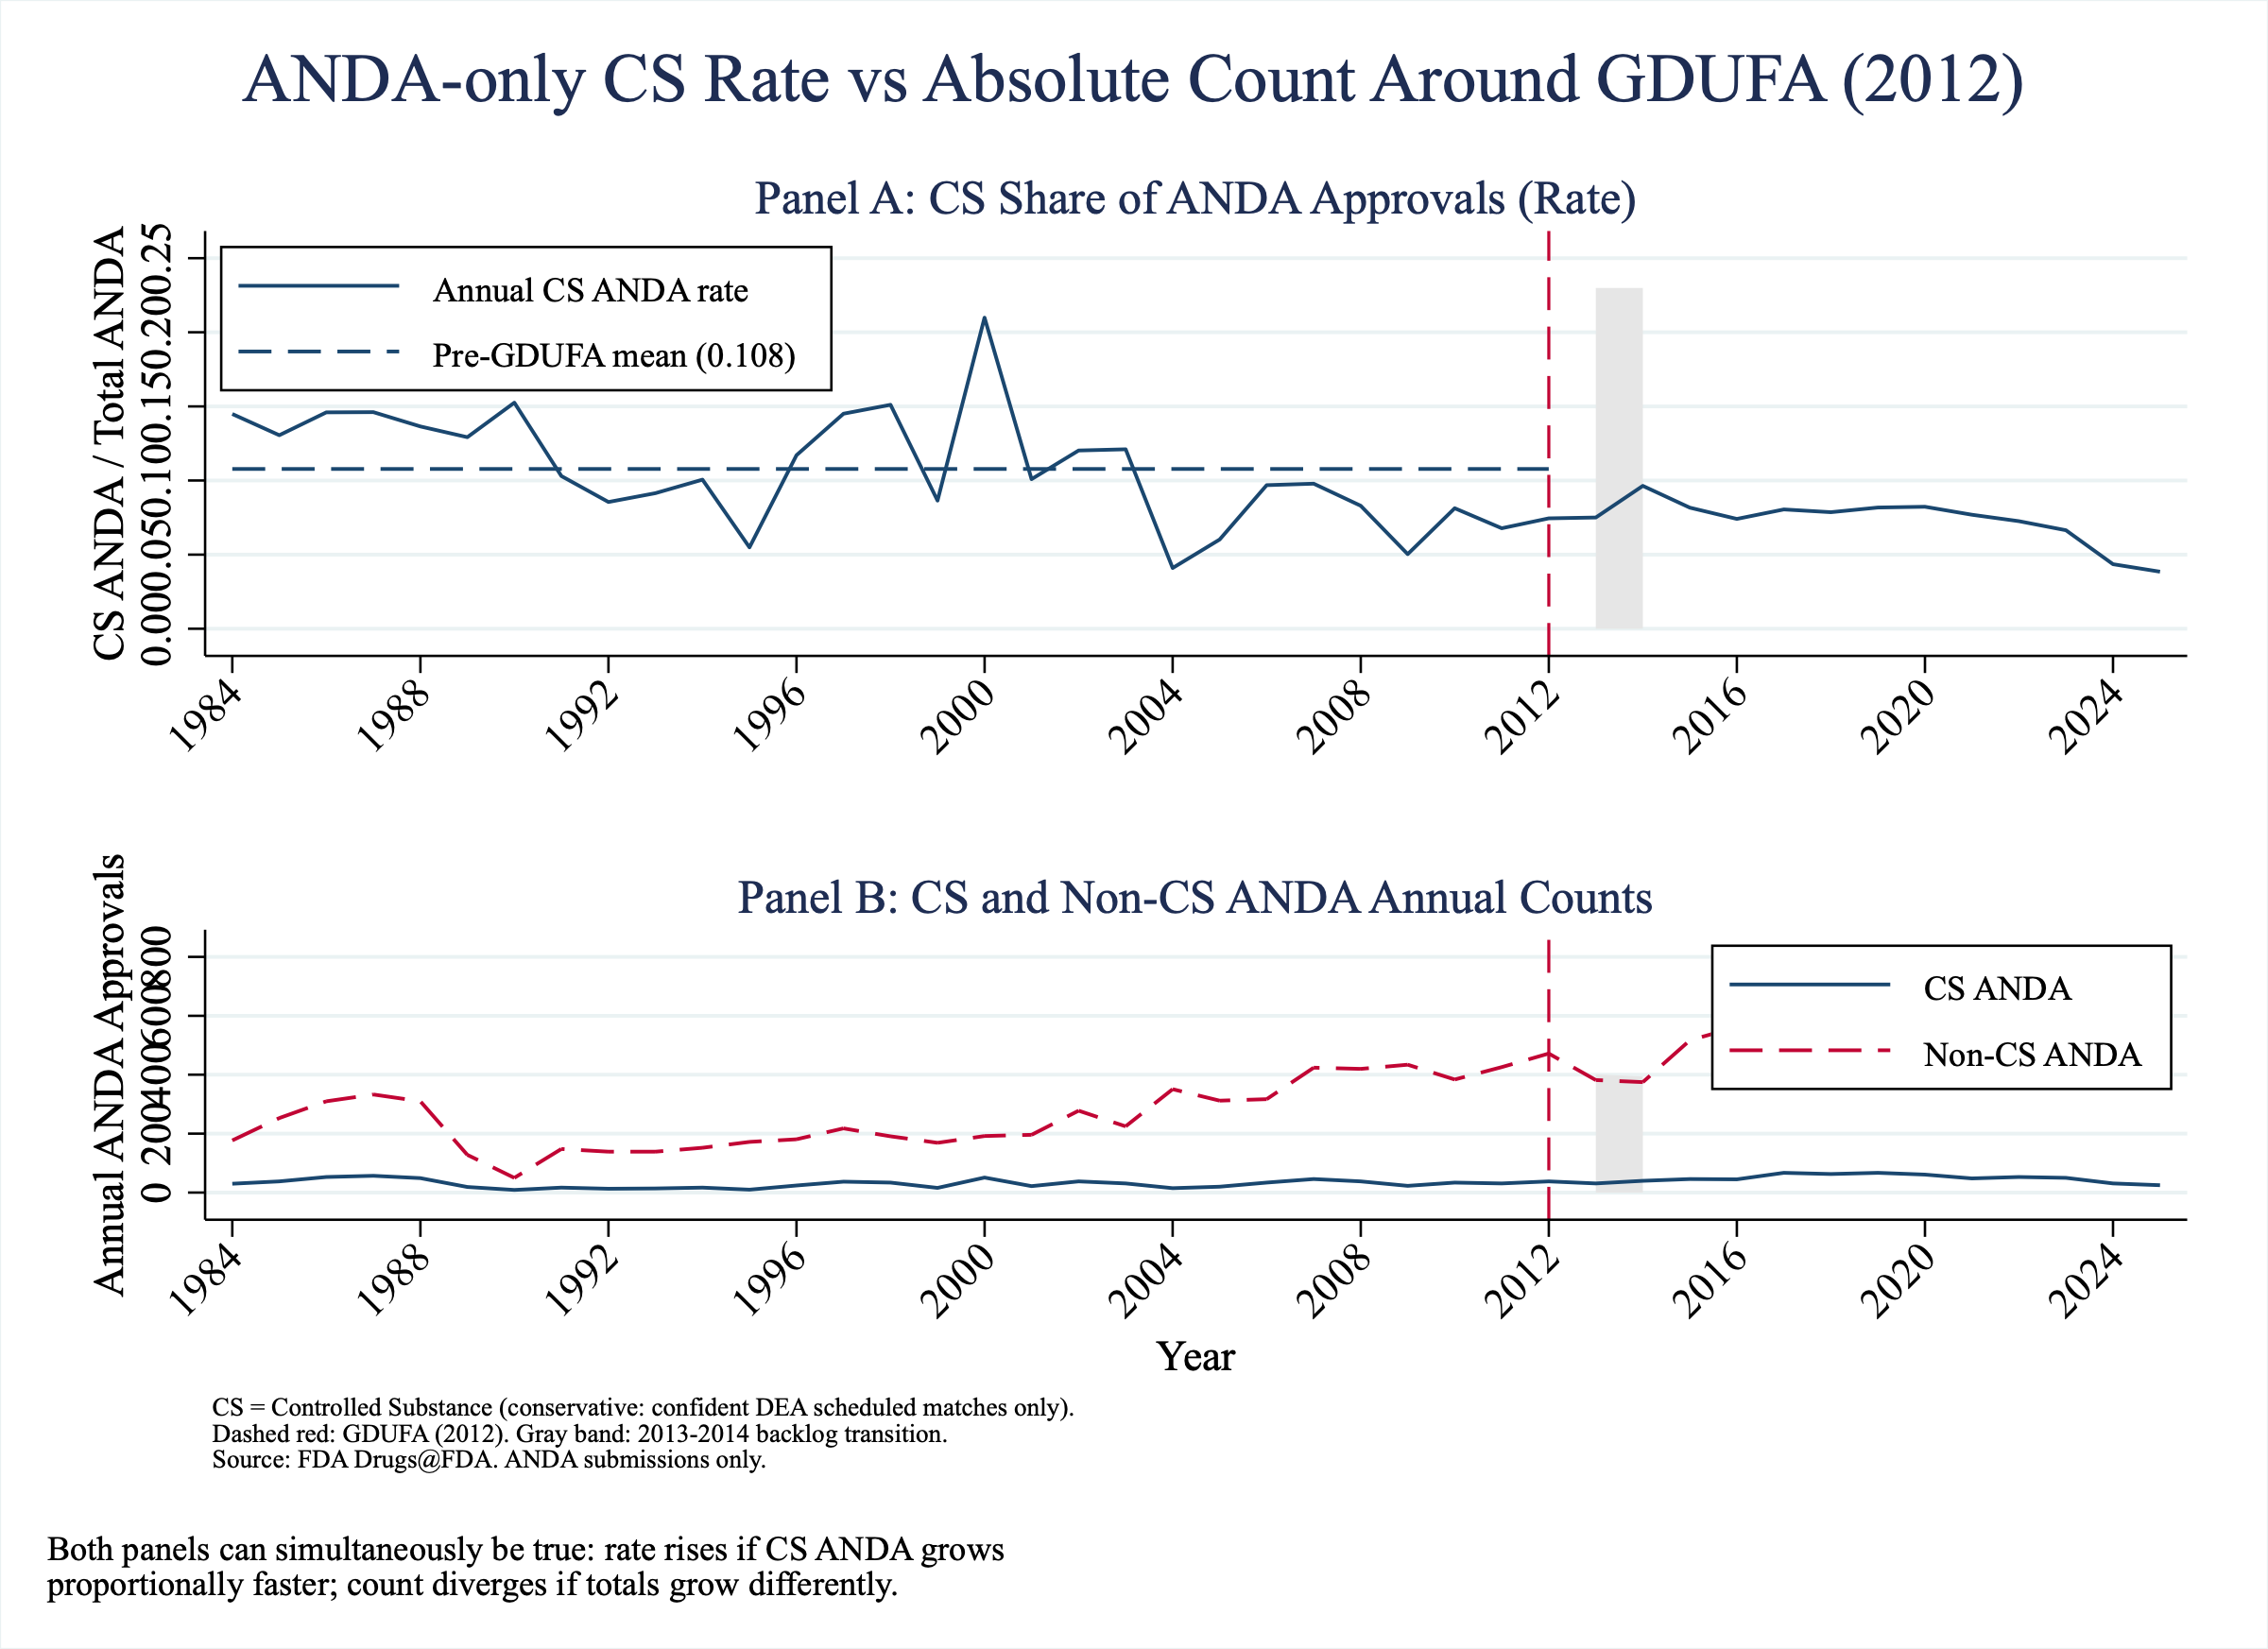
\includegraphics[width=0.92\textwidth]{../output/figures/stata/gdufa_anda_rate_vs_count.png}
\caption{GDUFA ANDA CS approvals: rate (Panel A) and absolute count (Panel B). Shaded region: 2013--2014 transition period.}
\label{fig:gdufa_rate_count}
\end{figure}

\begin{table}[htbp]
\centering
\begin{threeparttable}
\caption{GDUFA and PDUFA Stacked Poisson DD: Sensitivity to Trend Controls}
\label{tab:gdufa_results}
\small
\begin{tabular}{lcccc}
\toprule
 & Coef. & SE & IRR & 95\% CI \\
\midrule
\multicolumn{5}{l}{\textit{Panel A: GDUFA, ANDA-only}} \\
Year FE & $-0.403$ & $0.095$ & $0.668$ & $[0.55,\,0.81]$ \\
Linear trend & $-0.403$ & $0.152$ & $0.668$ & $[0.50,\,0.90]$ \\
Group-specific trends & $\phantom{-}0.323$ & $0.240$ & $1.382$ & $[0.86,\,2.21]$ \\
\midrule
\multicolumn{5}{l}{\textit{Panel B: PDUFA, NDA-only}} \\
Year FE & $\phantom{-}0.376$ & $0.200$ & $1.456$ & $[0.98,\,2.16]$ \\
Linear trend & $\phantom{-}0.376$ & $0.205$ & $1.456$ & $[0.97,\,2.18]$ \\
Group-specific trends & $\phantom{-}0.174$ & $0.356$ & $1.190$ & $[0.59,\,2.39]$ \\
\bottomrule
\end{tabular}
\begin{tablenotes}
\footnotesize
\item Stacked Poisson DD with log-total-approval exposure. Robust standard errors.
\item GDUFA excludes 2013--2014 transition years. PDUFA uses NDA-only sample.
\end{tablenotes}
\end{threeparttable}
\end{table}

\subsection{Sponsor Concentration}

Figure~\ref{fig:nda_hhi} and Figure~\ref{fig:gdufa_hhi} report Herfindahl--Hirschman Indices of sponsor concentration among CS NDA approvals (Figure~\ref{fig:nda_hhi}) and all ANDA approvals (Figure~\ref{fig:gdufa_hhi}). The CS NDA HHI is notably higher and more variable than the ANDA HHI, reflecting the smaller annual count of CS NDA approvals and the dominance of a small number of branded sponsors in certain years. The GDUFA era is associated with a visible decline in ANDA CS HHI, consistent with both the entry of additional generic sponsors and the decline in CS ANDA volume.

\begin{figure}[htbp]
\centering
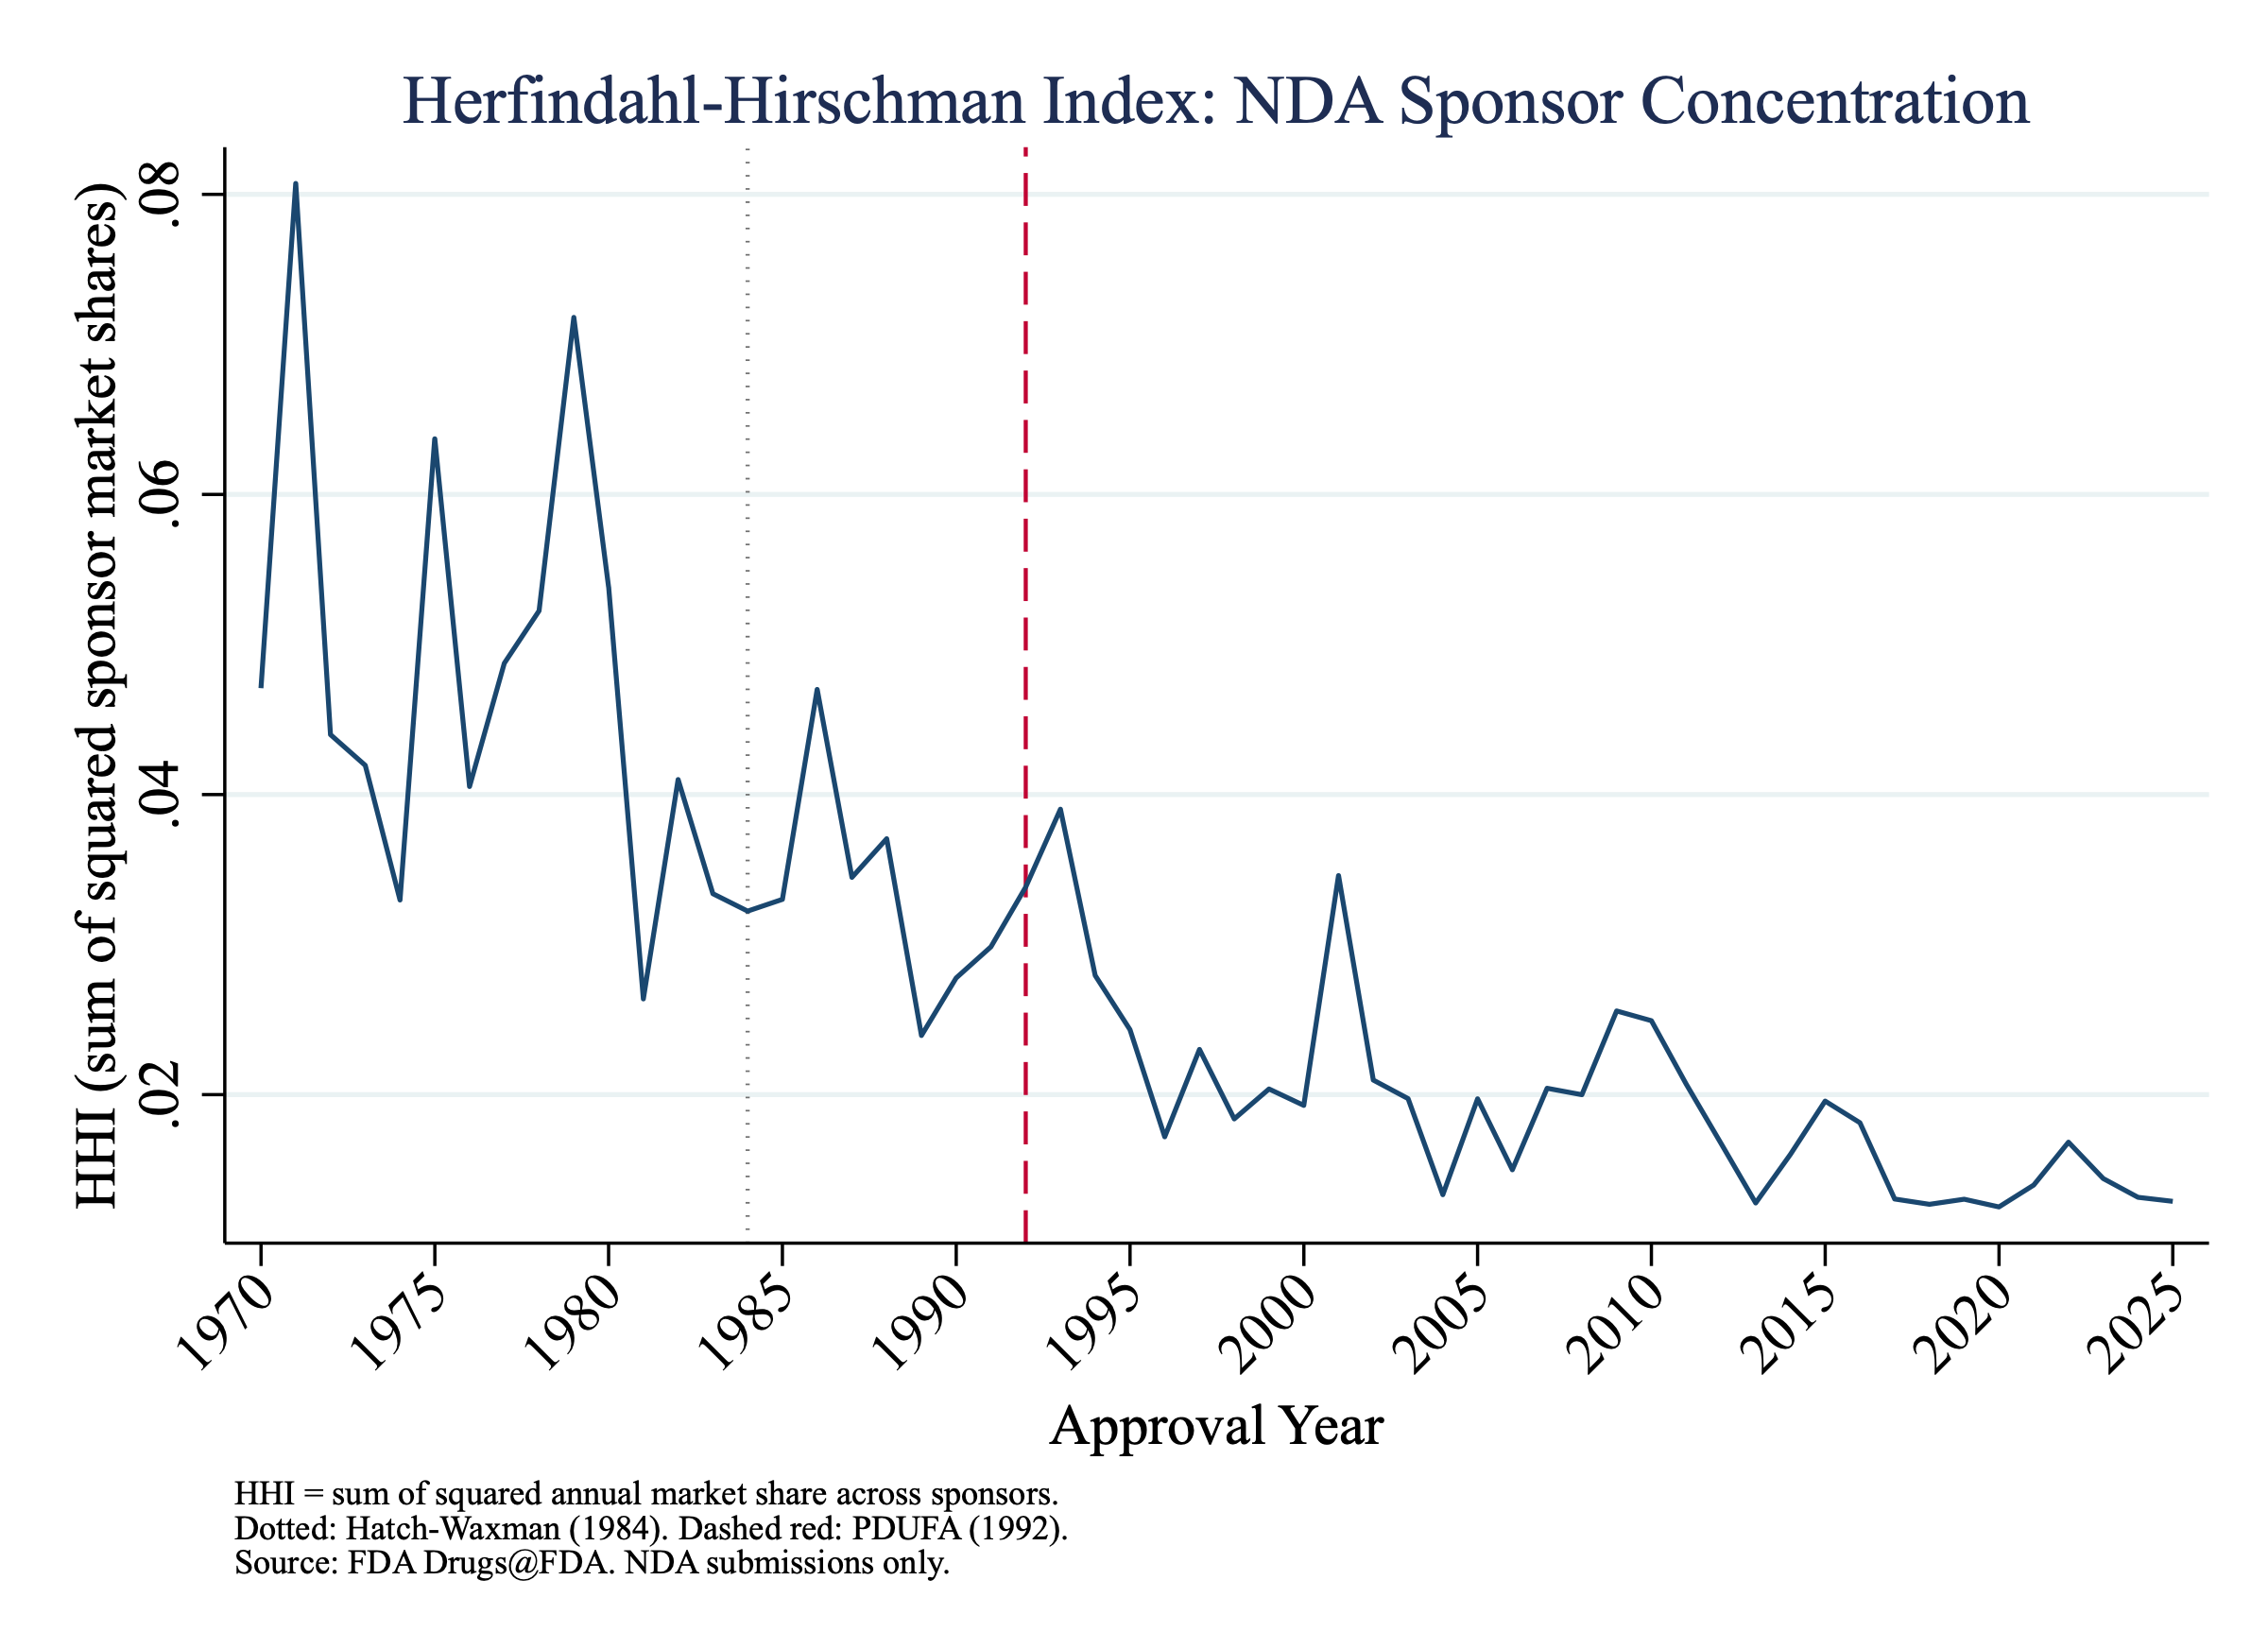
\includegraphics[width=0.92\textwidth]{../output/figures/stata/pdufa_nda_sponsor_concentration_hhi.png}
\caption{Sponsor HHI for CS NDA approvals, 1970--2025. Higher HHI = greater sponsor concentration. PDUFA reference lines marked.}
\label{fig:nda_hhi}
\end{figure}

\begin{figure}[htbp]
\centering
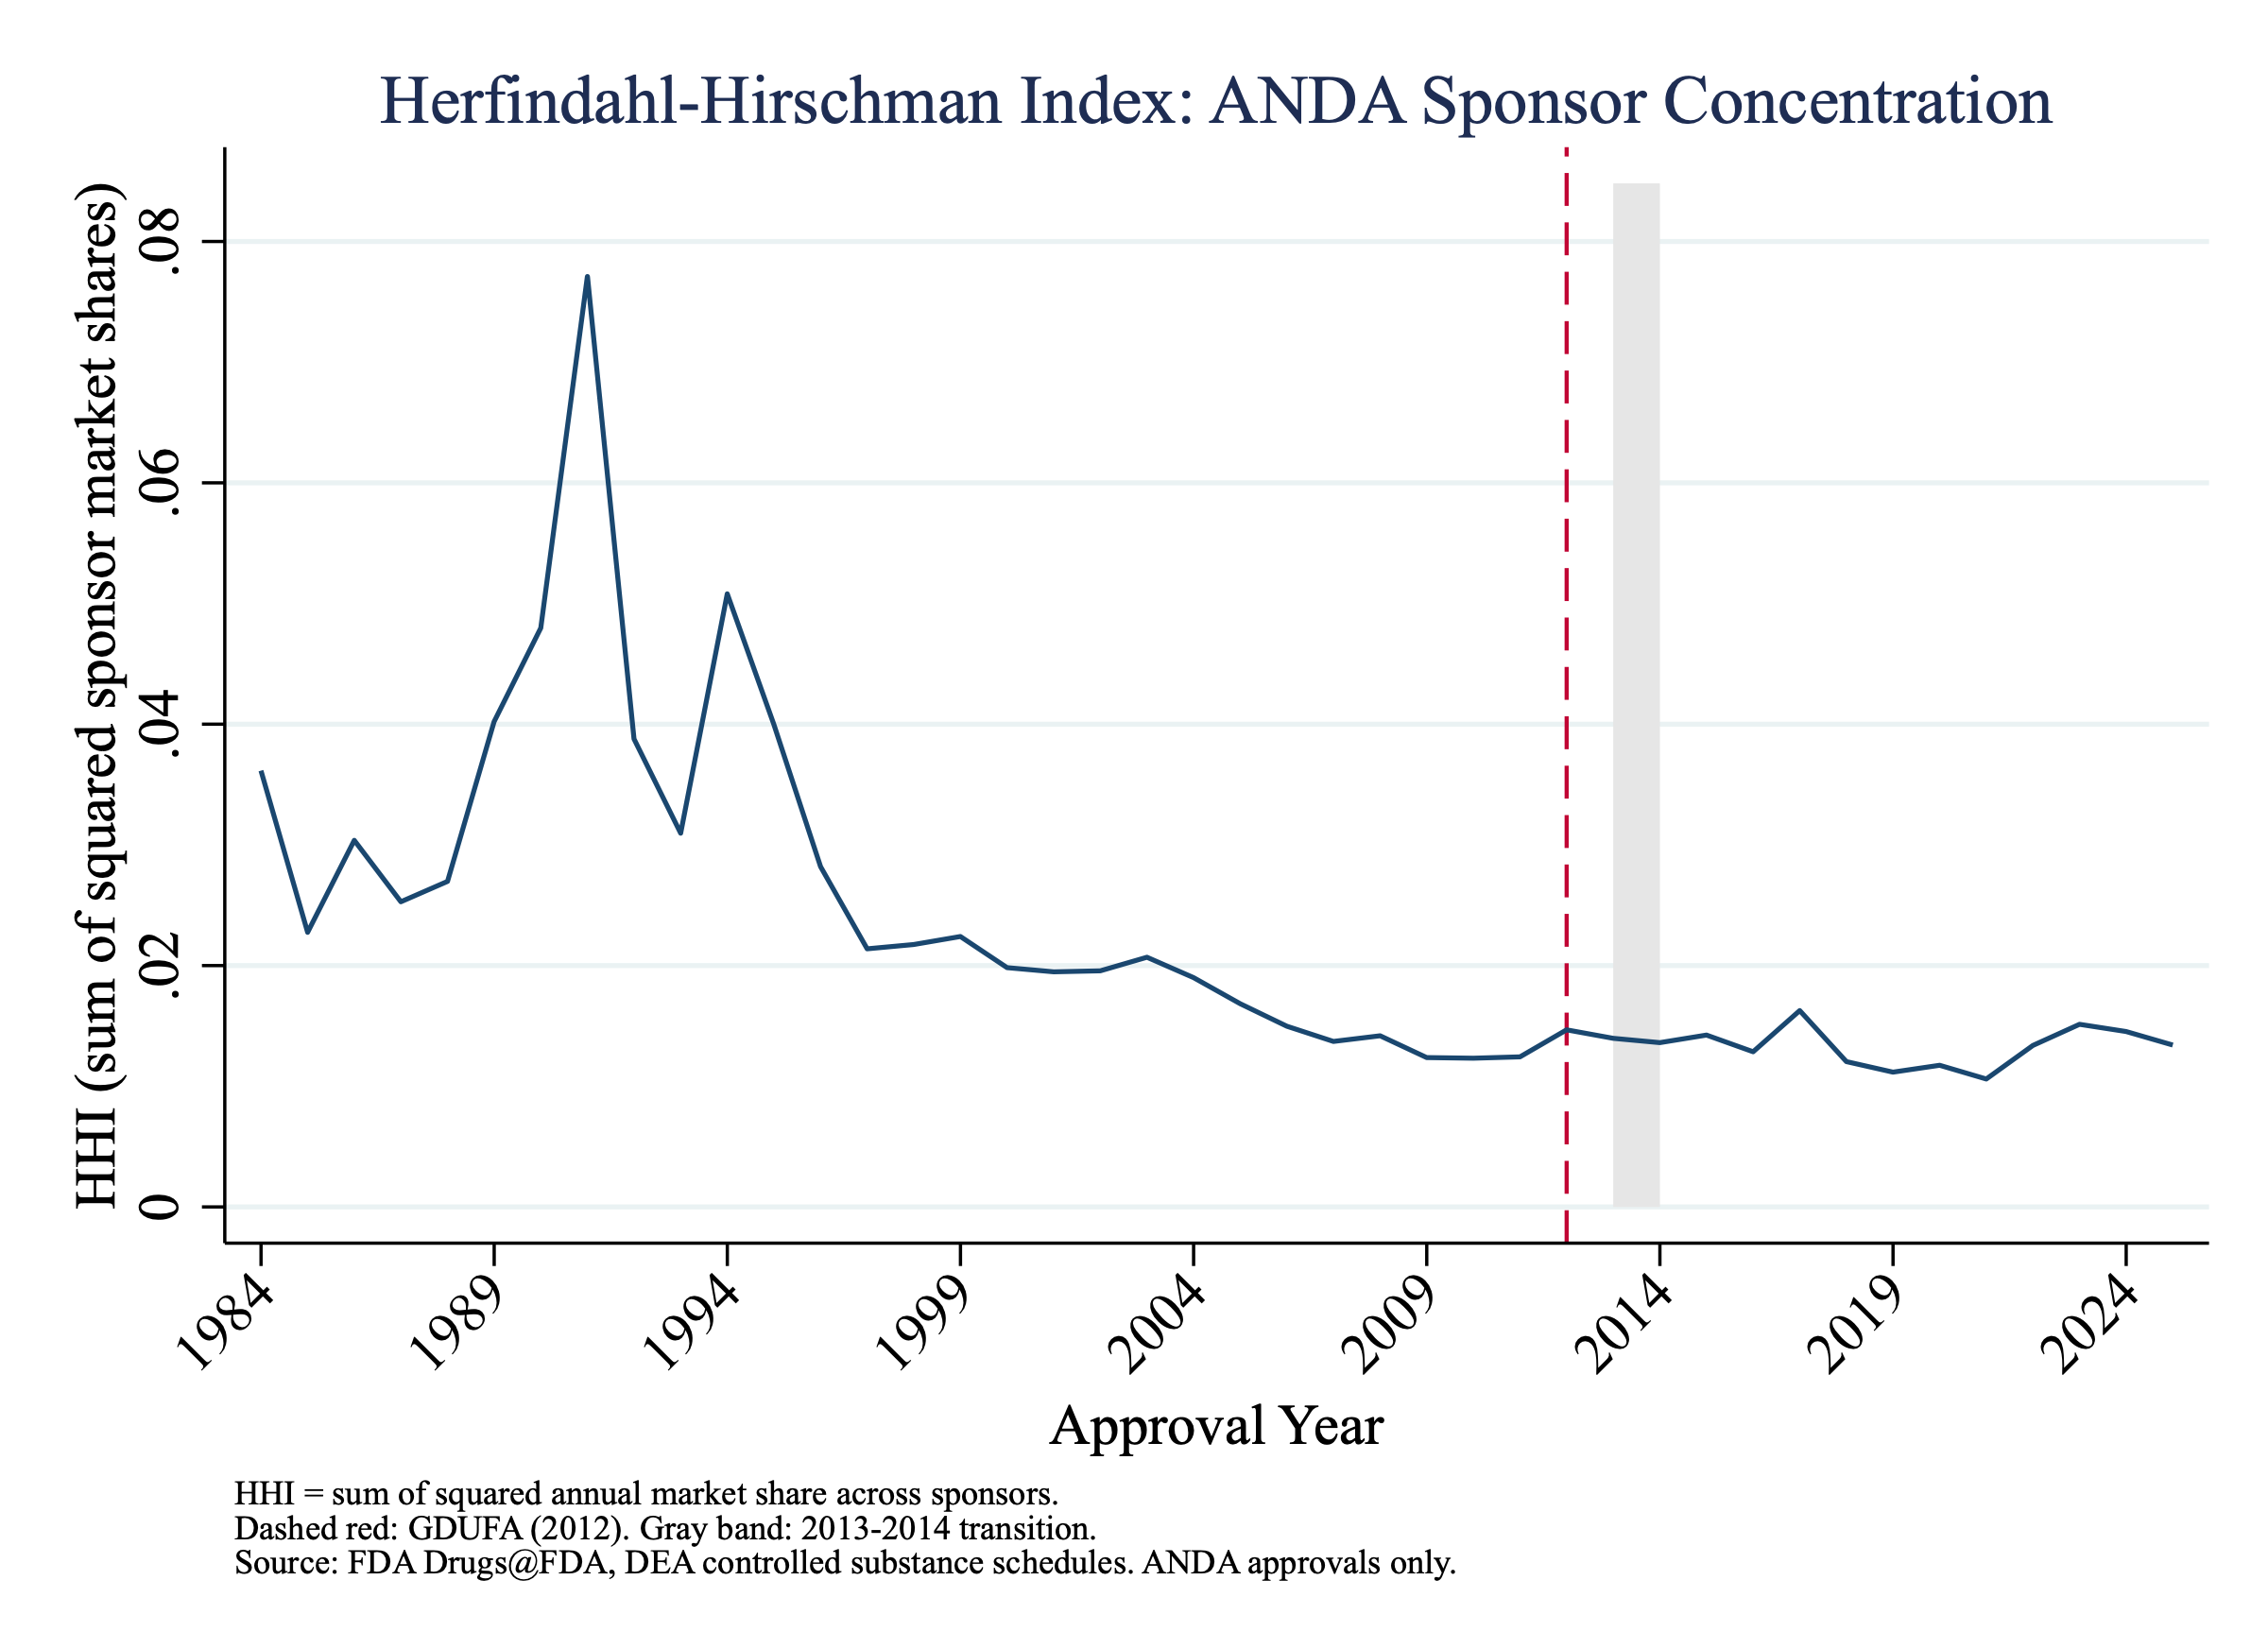
\includegraphics[width=0.92\textwidth]{../output/figures/stata/gdufa_sponsor_concentration_hhi.png}
\caption{Sponsor HHI for ANDA approvals (all), 1984--2025. GDUFA reference line marked.}
\label{fig:gdufa_hhi}
\end{figure}

Table~\ref{tab:top_sponsors} reports the top sponsors of CS NDA approvals over the full 1970--2025 period. The market is fragmented: the leading sponsors (HIKMA and UCB INC, tied at 9 CS NDAs each) account for only 4.1\% of the 222 CS NDAs in this window. Purdue Pharma LP ranks fourth with 7 approvals (3.2\%), reflecting both its historical dominance in branded opioid formulations and the relatively small absolute scale of any single sponsor's CS NDA portfolio.

\begin{table}[htbp]
\centering
\begin{threeparttable}
\caption{Top 10 Sponsors of CS NDA Approvals, 1970--2025}
\label{tab:top_sponsors}
\small
\begin{tabular}{llrr}
\toprule
Rank & Sponsor & CS NDAs & Share (\%) \\
\midrule
1 & HIKMA & 9 & 4.05 \\
1 & UCB INC & 9 & 4.05 \\
3 & SPECGX LLC & 7 & 3.15 \\
3 & PURDUE PHARMA LP & 7 & 3.15 \\
5 & INDIVIOR & 5 & 2.25 \\
5 & SANOFI AVENTIS US & 5 & 2.25 \\
5 & UPJOHN & 5 & 2.25 \\
8 & ABBOTT & 4 & 1.80 \\
8 & COLLEGIUM PHARM INC & 4 & 1.80 \\
8 & JANSSEN PHARMS & 4 & 1.80 \\
8 & TAKEDA PHARMS USA & 4 & 1.80 \\
\bottomrule
\end{tabular}
\begin{tablenotes}
\footnotesize
\item Universe: CS NDAs with confident DEA schedule match, 1970--2025, sponsor name non-missing.
\item Total CS NDAs in window: 222. Source: \texttt{cs\_nda\_top\_sponsors\_1970\_2025.csv}.
\end{tablenotes}
\end{threeparttable}
\end{table}

\section{Discussion}
\label{sec:discussion}

\subsection{Interpreting the Null}

The reduced-form evidence does not support the hypothesis that user-fee-funded review acceleration changed the controlled-substance composition of FDA approvals. The aggregate CS share fell after PDUFA. The NDA-only Poisson rate model returns an incidence-rate ratio of $1.46$ ($p = 0.06$) under year fixed effects, but the same coefficient collapses to $1.19$ with a 95\% confidence interval of $[0.59, 2.39]$ once group-specific linear trends are allowed. The GDUFA result follows the same pattern in the opposite direction: a year-FE IRR of $0.668$ that flips to $1.38$ with confidence interval $[0.86, 2.21]$ under group-specific trends. In both cases the most flexible specification places the user-fee composition effect in a band that includes both small reductions and small increases relative to the pre-policy baseline. The point estimates flip sign across specifications --- a feature, not a bug, of the data: the year-FE estimates are absorbing slow-moving differences in the CS and non-CS approval streams that have no plausible structural relationship to the user-fee policy enacted at the boundary year.

This is the right way to read the result. It is not that the data are too noisy to detect anything. It is that, once the empirical specification is allowed to accommodate the secular trends that pharmaceutical innovation followed during the 1980s and 2010s, no level shift remains to be explained by user-fee acceleration. The negative finding therefore does what a precisely estimated null can do in policy economics: it bounds the joint effect that any plausible mechanism --- demand-side incentives operating through the present-value channel of Section~\ref{sec:theory}, supply-side capacity expansion through additional FDA staffing, or any combination of the two --- could have produced through the approval-composition margin.

\subsection{The 2009--2013 Opioid Product Cycle as a Separable Phenomenon}

The drug-level evidence in Table~\ref{tab:spike_drugs} makes a stronger case for a separable explanation than for a delayed PDUFA effect. Three features matter. First, the timing --- seventeen to twenty-one years after PDUFA enactment --- is inconsistent with an immediate or even moderately delayed regulatory-incentive response. Second, the drugs themselves are recognizable products from the documented opioid product-innovation cycle: reformulated OxyContin, Exalgo, Embeda, Suboxone, Zohydro ER, and a cluster of branded testosterone formulations. Third, the spike subsides after 2013, suggesting a product-cycle dynamic rather than a permanent shift in approval composition.

The spike inflates post-PDUFA IRRs in specifications that do not allow group-specific trends because the pre-PDUFA NDA CS rate was low and the late-2000s wave creates a large mean difference in the post period that the simpler models then attribute to the policy variable. The fact that the group-specific-trend specification eliminates this elevation confirms the diagnosis: the late-2000s wave is doing the work that the post-PDUFA dummy was getting credit for.

This finding fits the broader opioid-supply literature. \textcite{alpertSupplySideDrugPolicy2018a} document that the branded opioid wave was followed by a substitution response in illicit markets; the approval-side documentation here provides complementary upstream evidence. The implication for policy is that the regulatory approval channel and the industry innovation channel are distinct: FDA approval decisions necessarily preceded each opioid wave product, but the timing and clustering of those products are not naturally explained by user-fee acceleration. The driver appears to be firm-level investment decisions about a specific high-margin therapeutic segment --- not the PDUFA review-time incentive structure operating uniformly across all NDA applications.

\subsection{Interpreting the GDUFA Result}

The year-FE GDUFA estimate, taken on its own, would imply a one-third decline in the CS share of ANDA approvals after the post-2015 performance-goal era. The direction is opposite to the regulatory-acceleration hypothesis: if faster review disproportionately benefited CS generics, the CS ANDA share should rise, not fall. But the headline year-FE result is not robust. The group-specific-trends specification yields an IRR of $1.38$ with a confidence interval of $[0.86, 2.21]$, which is statistically indistinguishable from one. The level decline observed under year fixed effects is absorbed once the analysis accommodates the long pre-period decline in the CS share of ANDA approvals --- a decline that is visible in the descriptive series in Section~\ref{sec:results_gdufa} and that began well before GDUFA.

Three substantive forces are consistent with this pre-existing decline. First, the pre-GDUFA ANDA backlog disproportionately included CS generics filed during the 1990s--2000s opioid expansion; clearing the backlog during 2013--2014 produced elevated CS ANDA approvals in the transition period and a subsequent reversion as the backlog drained. Second, the post-2012 ANDA filing pipeline shifted toward non-CS generics in response to the 2005--2012 patent cliff for non-opioid branded drugs, mechanically lowering the CS share of approvals as those generics cleared review. Third, the prescription opioid market contracted after 2012 as prescribing guidelines tightened, state prescription drug monitoring programs expanded, and supply-side interventions restricted access. Reduced demand for opioid generics may have discouraged new CS ANDA filings relative to non-CS filings independent of GDUFA. These three channels are observationally close to one another and to the user-fee channel, and the data here cannot separate them.

The right interpretation of the GDUFA result is therefore the same as the PDUFA result: under the most flexible specification, the user-fee composition effect is indistinguishable from zero, and the direction of the year-FE point estimate provides little additional information once the slower-moving secular movement in the CS-ANDA share is allowed to load on its own trend.

\subsection{Limitations and Future Work}

Several limitations constrain the conclusions. The most important is the DEA linkage: because current schedules are used rather than historical schedules, drugs that were scheduled or rescheduled after their FDA approval date are misclassified. The conservative-match definition concentrates the linkage on substances that have been continuously scheduled for decades, which limits the practical extent of the bias, but the direction of any residual error for the main results is unclear. A second limitation is the single national time series, which provides limited statistical power and cannot separate the user-fee channel from contemporaneous secular trends in pharmaceutical innovation. A third limitation is the absence of a downstream outcome: this paper characterizes the approval-side composition of CS drugs but does not measure downstream prescribing volume, misuse, or diversion.

Four directions follow naturally for future work. First, constructing a historical DEA scheduling database would allow each drug to be classified by its schedule as of its approval date, eliminating the retroactive-linkage limitation. Second, linking approval-side CS counts to prescribing data from sources such as IQVIA or ARCOS would estimate the downstream supply implications of any composition change, even if that change is small. Third, extending the GDUFA analysis to GDUFA II and III as those program years accumulate will provide additional post-treatment observations and may sharpen the identification. Fourth, exploiting therapeutic-class or firm-level variation could begin to separate the demand-side incentive channel from the supply-side capacity channel within the user-fee mechanism, distinguishing the two competing theoretical accounts in Section~\ref{sec:theory}.

\section{Conclusion}
\label{sec:conclusion}

This paper asks whether PDUFA (1992) and GDUFA (2012) --- the two major user-fee-funded regulatory acceleration reforms at the FDA --- changed the controlled-substance share of original drug approvals. Using the complete Drugs@FDA database from 1939 through 2025 ($N = 25{,}908$) linked to DEA scheduling records, I estimate share-based interrupted time series, Poisson rate models with exposure, and stacked difference-in-differences specifications for both the NDA pathway (PDUFA) and the ANDA pathway (GDUFA), and supplement these with rate-versus-count diagnostics, group-specific linear time trends, and event-study DD designs.

The central finding is a precisely estimated null. In the most flexible specifications, the post-policy incidence-rate ratio for the controlled-substance share is $1.19$ for PDUFA on the NDA pathway (95\% CI $[0.59, 2.39]$) and $1.38$ for GDUFA on the ANDA pathway (95\% CI $[0.86, 2.21]$). The point estimates flip sign between less and more flexible specifications, which is itself diagnostic: when the empirical model is allowed to absorb the slow-moving secular movements in the CS and non-CS approval streams that have no plausible structural relationship to the user-fee policy variable, no level shift remains for that variable to explain. The apparent post-PDUFA NDA elevation in less flexible specifications is traceable to a separable late-2000s wave of branded extended-release and abuse-deterrent opioid formulations approved seventeen to twenty-one years after PDUFA enactment.

The findings carry two implications. First, the standard economic prediction --- that user-fee-funded review acceleration should disproportionately benefit drug classes with the largest expected revenue streams, including controlled substances --- does not find approval-side support in the data. The compositional variation that does exist is better explained by industry product cycles, post-Hatch--Waxman ANDA expansion, and the demand environment for prescription opioids than by review-time incentives at the regulatory margin. Second, this is not the same as saying that FDA regulatory policy is irrelevant to the controlled-substance supply chain. Approval is a necessary condition for market entry, and every product on the list in Table~\ref{tab:spike_drugs} required FDA clearance before it could reach prescribers. What the data do not support is the upstream causal chain from user-fee acceleration to approval composition.

For researchers and policymakers, the takeaway is that the causal pathway from regulatory acceleration to controlled-substance supply, if it exists, runs primarily through the innovation-investment channel --- firms deciding whether to develop CS products --- rather than through the review-time channel. Understanding that investment decision and how factors such as patent term, market exclusivity, and prescribing-market demand conditions shape it is likely to be more productive for policy design than further refinements to FDA review-time performance goals. Future work that links the upstream approval-side evidence reported here to downstream prescribing volumes and ultimately to health outcomes will provide a more complete picture of how pharmaceutical regulation shapes controlled-substance supply across the full market chain.


\printbibliography

\appendix
\section{Appendix}
% add any additional tables, figures, or information that is relevant to the thesis but not essential to the main text. This can include detailed data descriptions, additional analyses, or supplementary materials. Each appendix should be labeled (e.g., Appendix A, Appendix B) and referenced in the main text where appropriate.


\printtodos

\end{document}
